\documentclass[10pt,a4paper,fleqn]{article}
\usepackage[utf8]{inputenc}
\usepackage{amsmath}
\usepackage{amsfonts}
\usepackage{amssymb}
\usepackage{graphicx}
\usepackage[left=2cm,right=2cm,top=2cm,bottom=2cm]{geometry}
\usepackage[hidelinks]{hyperref}
\usepackage[naustrian]{babel}
\usepackage{csquotes}
\MakeOuterQuote{"}
\begin{document}
\setlength{\mathindent}{2cm}% you can set it back to 0cm (the default).
	\begin{titlepage}
\newgeometry{left=3cm,right=1cm,bottom=0.1cm}
\newgeometry{bottom=1.5cm, top=1.5cm}
\sffamily

\begin{center}
	Nikolai KRAUS \\
  	\vspace{1cm}
  	\Large
  	\textbf{Klinische Medizin} \\
  	\vspace{0.5cm}
  	\normalsize
  	\vspace{0.5cm}
  	Folien und Mitschrift \\ 
  	Wintersemester 2014/15 \\
  	\url{https://bitbucket.org/Arkonos/km}
\end{center}
\end{titlepage}
\clearpage
	\tableofcontents
	\section{Allgemeine Krankheitslehre}

\subsection{Lehrinhalte "klinische Medizin"}
	\begin{itemize}
		\item \textbf{allgemeine Grundlagen der Krankheitslehre}
		\item \textbf{häufige Erkrankungen im Detail}
		\item \textbf{Diagnostik}
		\item \textbf{Therapie}
	\end{itemize}

\subsection{allgemeine Pathologie}
	\begin{itemize}
		\item \textbf{Definition}
			\begin{itemize}
				\item \textbf{Pathos, Logos}
				\item \textbf{Lehre von den Krankheiten (ihren Ursachen und den  Veränderungen, die sie im Organismus hervorrufen)}
			\end{itemize}
		\item \textbf{Ätiologie}
			\begin{itemize}
				\item \textbf{Lehre von den Krankheitsursachen}
			\end{itemize}
		\item \textbf{Pathogenese}
			\begin{itemize}
				\item \textbf{Lehre von der Entstehung einer Krankheit}
				\item Überleitung ins Detail. Ätiologie ist im Allgemeinen, während die Pathogenese schon mehr ins Detail geht.
			\end{itemize}
	\end{itemize}

\subsection{Epidemiologie}
	\begin{itemize}
		\item Die Verteilung des Krankheitsauftreten geographisch, demopgraphisch und zeitlich.
		\item \textbf{ursprüngliche Bedeutung: "Seuchenkunde"}
		\item \textbf{WHO Definition}
			\begin{itemize}
				\item \textbf{die Epidemiologie befasst sich mit der Untersuchung der Verteilung von Krankheiten, physiologischen Variablen und sozialen Krankheitsfolgen in menschlichen Bevölkerungsgruppen sowie mit Faktoren, die diese Verteilung beeinflussen}
				\item \textbf{Begriffsdefinitionen}
					\begin{itemize}
						\item \textbf{Gesundheit, Krankheit}
						\item \textbf{Morbidität, Mortalität, Letalität}
						\item \textbf{Inzidenz, Prävalenz}
					\end{itemize}
			\end{itemize}
		\item \textbf{Gesundheit}
			\begin{itemize}
				\item \textbf{Zustand völligen körperlichen, seelischen und sozialen Wohlbefindens}
				\item "paradisischer Zustand" unerreichbar, absolut perfekt
				\item Gesunheit - Krankheit fließender Übergang. In welchem Zustand man sich befindet liegt im Blickwinkel des Betrachters: Arzt. Patient
			\end{itemize}
		\item \textbf{Krankheit}
			\begin{itemize}
				\item \textbf{Störung in diesem körperlich-seelisch-geistig-sozialen Gleichgewicht}
			\end{itemize}
		\item \textbf{Morbidität} (Mobrid, lat - krank)
			\begin{itemize}
				\item \textbf{Häufigkeit einer bestimmten Krankheit in einer Bevölkerungsgruppe}
				\item \textbf{Verhältnis der Zahl der Erkrankungen zur Zahl der Gesamtbevölkerung in einem bestimmten Zeitraum}, meist pro Jahr
			\end{itemize}
		\item \textbf{Mortalität ("Sterblichkeit")} (mortal, lat - tödlich)
			\begin{itemize}
				\item \textbf{Häufigkeit einer bestimmten Krankheit als Todesursache in einer Bevölkerungsgruppe}
				\item \textbf{Verhältnis der Zahl der Todesfälle an bestimmter Erkrankung zur Zahl der Gesamtbevölkerung in einem bestimmten Zeitraum, in der Regel 1 Jahr, pro 10k Einwohner}
			\end{itemize}
	\pagebreak
		\item \textbf{Letalität ("Tödlichkeit")}
			\begin{itemize}
				\item \textbf{Zahl der Todesfälle bezogen auf die Zahl der Erkrankten}
				\item \textbf{Verhältnis der Zahl der Todesfälle zur Zahl der an einer bestimmten Krankheit Erkrankten ("Mortalität in \%")}
			\end{itemize}
		\item Beispiel Bauchspeicheldrüsenkrebs
			\begin{itemize}
				\item Mortalität sehr gering, Letalität extrem hoch
			\end{itemize}
		\item \textbf{Inzidenz (Erkrankungshäufigkeit)} (Inzidere, lat - Neubeginn)
			\begin{itemize}
				\item \textbf{Zahl von Neuerkrankungen an einer bestimmten Krankheit innerhalb eines bestimmten Zeitraumes}
				\item \textbf{Anzahl der Personen, die im Verlauf eines bestimmten Zeitraumes (i.d.R. 1 Jahr) an einer bestimmten Krankheit erstmals erkranken}
				\item Nimmt das in einer bestimmten Region zu? $\rightarrow$ der Ursache nachgehen
			\end{itemize}
		\item \textbf{Prävalenz}
			\begin{itemize}
				\item \textbf{Zahl der zu einem bestimmten Zeitpunkt an einer bestimmten Krankheit leidenden Personen, bezogen auf die Gesamtbevölkerung}
				\item Bsp.: Grippeninfektion im Januar deutlich höher als im August
			\end{itemize}
	\end{itemize}

\subsection{Methoden der pathologischen Diagnostik}
	\begin{itemize}
		\item u.a. Gerichtsmedizin
		\item \textbf{intravitale Diagnostik} auch am lebenden Gewebe
			\begin{itemize}
				\item \textbf{zytologische Untersuchungsmethoden}
				\item \textbf{histologische Untersuchungsmethoden}
			\end{itemize}
		\item \textbf{postmortale Diagnostik}
			\begin{itemize}
				\item \textbf{sanitätspolizeiliche Obduktion}
				\item \textbf{gerichtsmedizinische Obduktion}
				\item \textbf{klinische Obduktion}
			\end{itemize}
	\end{itemize}

\subsubsection{intravitale Diagnostik}
	\begin{itemize}
		\item \textbf{zytologische Untersuchungsmethoden}
			\begin{itemize}
				\item \textbf{Analyse von Einzelzellen}
				\item \textbf{Gewinnung der Zellen}
					\begin{itemize}
						\item \textbf{von Schleimhautoberflächen, Sekreten, Spülflüssigkeiten}
							\begin{itemize}
								\item Abstrichbeispiel: optimal Papanicolaou: Pap - Diagnose im Gebärmutterhals zur Diagnose von Krebs. Nicht sonderlich invasiv, kostengünstig, sehr aussagekräftig.
							\end{itemize}
						\item \textbf{durch Punktion von Flüssigkeiten}
							\begin{itemize}
								\item Entnahme von Sekreten. Einspritzen und Ausspülen und anschließende Analyse der Flüssigkeit in Organen
							\end{itemize}
						\item \textbf{durch Feinnadelpunktion von Organen}
							\begin{itemize}
								\item "pflücken" von Zellen mit einer Feinnadel
							\end{itemize}
					\end{itemize}
				\item \textbf{Zweck / häufige Fragestellungen}
					\begin{itemize}
						\item \textbf{infektiöse Erkrankungen (Erregernachweis) und deren Folgen}
						\item \textbf{Entzündungsdiagnostik}
						\item \textbf{Tumorzellnachweis}
						\item \textbf{$\dots$}
					\end{itemize}
			\end{itemize}
\pagebreak
		\item \textbf{histologische Untersuchungsmethoden}
			\begin{itemize}
				\item \textbf{Analyse von Gewebeschnitten von chirurgisch oder bioptisch gewonnenen Gewebestücken}
				\item \textbf{Gefrierschnellschnitt, Paraffinschnitt}
					\begin{itemize}
						\item Parafinschnitte sehr haltbar und aussagekräftiger als Gefrierschnitt
						\item Parafinschnitt 3-4 Tage, Gerierschnitt 15 Minuten
					\end{itemize}
				\item \textbf{Analysetechniken}
					\begin{itemize}
						\item \textbf{Lichtmikroskopie}
							\begin{itemize}
								\item \textbf{Anfertigung von Paraffinschnitten oder Gefrierschnitten}
							\end{itemize}
						\item \textbf{Immunfluoreszenz}
						\item \textbf{Elektronenmikroskopie}
					\end{itemize}
				\item \textbf{Zweck / häufige Fragestellungen}
					\begin{itemize}
						\item \textbf{Zellbeurteilung im Gewebeverband}
						\item \textbf{Tumordiagnostik}
						\item \textbf{Kontrolle des chirurgischen Eingriffs (Resektionsränder)}
						\item \textbf{$\dots$}
					\end{itemize}
				\item kleine Gewebsentnahme - Biopsi (Probexcision - PE)
				\item große Entfernungen - Operation (Resektion)
				\item[1.] Biopsie
				\item[2.] Pathologische Aufbearbeitung - Aufschneiden in feinste, dünnste Schnitte 
				\item[] (für rasche Diagnose: Rohrpost - bsp. während einer Tumoroperation. Wo endet der Tumor, wo beginnt gesundes Gewebe, anschließendes Warten auf die Rückmeldung 
			\end{itemize}
			\begin{center}
				\includegraphics[scale=0.7]{{klin.med.-grundlagen-img0000}.png}
			\end{center}
\pagebreak
		\item \textbf{bakteriologische und serologische Diagnostik}
			\begin{itemize}
				\item direkt oder indirekt: Entweder direkt den Erreger, oder indirekt durch den Nachweis von gehäuften Auftreten der Antikörper
				\item \textbf{mikroskopischer Nachweis von Krankheitserregern}
					\begin{itemize}
						\item \textbf{spezielle Färbemethoden zur Darstellung der Mikroorganismen}
							\begin{itemize}
								\item \textbf{Lichtmikroskopie}
								\item \textbf{Elektronenmikroskopie}
							\end{itemize}
					\end{itemize}
				\item \textbf{kultureller Nachweis von Krankheitserregern}
					\begin{itemize}
						\item \textbf{Bakterienkultur auf flüssigen oder festen Nährmedien} (Zucht)
					\end{itemize}
				\item \textbf{serologischer Nachweis von Krankheitserregern}
					\begin{itemize}
						\item \textbf{Antigen-Antikörper-Reaktion}
						\item \textbf{Agglutinationsreaktionen}
							\begin{itemize}
								\item \textbf{Antigen-Suchtest}
								\item \textbf{Antikörper-Suchtest}
								\item mit freiem Auge sichtbar - Flockig, körnig
								\item Bsp.: Zusammentreffen von unterschiedlichen Blutgruppen
							\end{itemize}
					\end{itemize}
			\end{itemize}
		\item \textbf{Spezialmethoden}
			\begin{itemize}
				\item \textbf{Elektronenmikroskopie}
					\begin{itemize}
						\item Details innerhalb der Zelle, wird zunehmend ersetzt durch unten angeführte Verfahren
					\end{itemize}
				\item \textbf{Immunhistochemie}
					\begin{itemize}
						\item \textbf{Sichtbarmachen spezieller Zell- und Gewebe-Strukturen durch spezifische AG-AK-Reaktionen mittels monoklonaler AK}
						\item Markierung mit Fluoreszenzfarbstoffen
					\end{itemize}
				\item \textbf{biochemische Untersuchungen}
					\begin{itemize}
						\item Proteinnachweis, Viren, Kohlenhydrate, Medikamente
						\item \textbf{Nachweis bestimmter Strukturen aus Körperflüssigkeiten}, wieder mittels Markierung (radioaktiv)
						\item \textbf{Techniken: Immuno-Assay, Blotting-Verfahren (Immunoblot)}, Antikörper - Antigenreaktion + Visualisierung
					\end{itemize}
				\item \textbf{molekularbiologische Techniken}
					\begin{itemize}
						\item \textbf{Hybridisierungsmethoden}
							\begin{itemize}
								\item Hybridisierung - Aneinanderlegen der Nukleinsäuresequenzen
								\item zB.: Virus DNA - Nachweiß von Virusbefall, Tumore
							\end{itemize}
						\item \textbf{Amplifizierungsmethoden}
							\begin{itemize}
								\item Vermehrung von DNA Proben mit Polimerase Kettenreaktion (PCR - Polymerase Chainreaction)
							\end{itemize}
					\end{itemize}
		\end{itemize}
	\end{itemize}

\pagebreak
\subsubsection{postmortale Diagnostik}
	\begin{itemize}
		\item \textbf{Obduktion, Sektion (lat, schneiden), innere Leichenbeschau, Autopsie}
			\begin{itemize}
				\item \textbf{sanitätspolizeiliche Obduktion}
					\begin{itemize}
						\item \textbf{bei ungenügender Information}
						\item Bei Versterben zu Hause; Leiche begutachten (überprüfen eines natürlichen Todes) und für die Bestattung freigeben
					\end{itemize}
				\item \textbf{gerichtsmedizinische Obduktion}
					\begin{itemize}
						\item \textbf{bei Verdacht auf Fremdverschulden}
					\end{itemize}
				\item \textbf{klinische Obduktion}
					\begin{itemize}
						\item \textbf{zur Qualitätskontrolle}
						\item Rückmeldung an die Ärzte, ob sie mit ihrer Diagnose richtig lagen, für Lehre und Ausbildung von Jungmedizinern.
						\item Zwingend nach operativen Eingriff mit Todesfolge
					\end{itemize}
				\item Obduktionen können auch angefordert werden - Versicherungen
				\item \textbf{Zweck}
					\begin{itemize}
						\item \textbf{Grundlage für Statistiken und gesundheitspolitische Maßnahmen}
						\item \textbf{wissenschaftliche Aufgaben}
						\item \textbf{rechtliche Grundlagen siehe Krankenanstaltengesetz}
					\end{itemize}
			\end{itemize}
	\end{itemize}

\subsection{Krankheitsursachen, -Verlauf, -Ausgang}
\subsubsection{Übersicht}
	\begin{itemize}
		\item \textbf{Krankheitsursachen (Ätiologie)}
			\begin{itemize}
				\item \textbf{endogene Krankheitsursachen}
				\item \textbf{exogene Krankheitsursachen}
				\item Ursache im, oder außerhalb des Körpers
			\end{itemize}
		\item \textbf{Krankheitsverlauf}
			\begin{itemize}
				\item \textbf{nach zeitlichem Verlauf}
				\item \textbf{Rezidiv, Remission}
			\end{itemize}
		\item \textbf{Krankheitsausgang}
	\end{itemize}

\subsubsection{Krankheitsursachen}
	\begin{itemize}
		\item \textbf{innere (endogene) Krankheitsursachen}
			\begin{itemize}
				\item \textbf{genetische Störungen}
					\begin{itemize}
						\item \textbf{Chromosomenschäden, DNA-Schäden}
						\item zB.: durch radioaktive Bestrahlung
					\end{itemize}
				\item \textbf{Disposition} (Krankheitsneigung, erhöhtes Risiko, erhöhte Wahrscheinlichkeit)
					\begin{itemize}
						\item \textbf{Altersdisposition} (Kinderkrankheiten)
						\item \textbf{Geschlechtsdisposition} (Brustkrebs - weiblich)
						\item \textbf{genetische Disposition}
						\item \textbf{pathologische Disposition}
						\item eine Krankheit legt den Grundstein für eine andere Erkrankung
						\item HIV nicht nur Disposition, da absoluter Garant für Erkrankung
						\item Bsp.: krankheitliche Vernarbung des Darms führt zu erhöhter Infektionsgefahr 
					\end{itemize}
				\item \textbf{Autoimmunerkrankungen}
					\begin{itemize}
						\item Das Immunsystem zerstört irrtümlich gutartiges Gewebe, Zellen
					\end{itemize}
				\item \textbf{hormonelle (endokrine) Störungen}
			\end{itemize}
\pagebreak
		\item \textbf{äußere (exogene) Krankheitsursachen}
			\begin{itemize}
				\item \textbf{Noxen} (lat, schädigende Einwirkung)
					\begin{itemize}
						\item \textbf{eine Noxe ist eine Substanz oder ein Ereignis, das einem biologischen Organismus Schäden zufügt}
						\item \textbf{im weiteren Sinn versteht man unter einer "Noxe" jede Art von äußerer Krankheitsursache}
					\end{itemize}
			\end{itemize}
	\end{itemize}
\paragraph{Krankheitsursachen - Noxen}
	\begin{itemize}
		\item \textbf{physikalische Noxen}
			\begin{itemize}
				\item \textbf{mechanische Einwirkung}
					\begin{itemize}
						\item \textbf{akut: Trauma (Quetschung, Schnitt, Druck: Barotrauma, $\dots$)}
						\item \textbf{chronisch: Dekubitus}
							\begin{itemize}
								\item Auch Druck - reine Schwerkraftswirkung: zB.: Wundlegen bei Patienten
							\end{itemize}
						\item Schleudertrauma - Zerrung von Muskeln und Bändern im Halsbereich
					\end{itemize}
				\item \textbf{thermische Einwirkung}
					\begin{itemize}
						\item \textbf{Verbrennungen}
						\item \textbf{Erfrierungen}
					\end{itemize}
				\item \textbf{Luftdruckveränderungen}
					\begin{itemize}
						\item \textbf{Höhenkrankheit}
						\item \textbf{Dekompressionssyndrom}
						\item Blut: 3 verschiedene Substanzen
						\item Erythrozyten (Roter Blutfarbstoff - Hämoglobin am Eisen - O$_2$) - Mangel = Anemie $\rightarrow$ Müdigkeit, Depressionen
						\item Bei Höhenkrankheit: Hyperventilation, Tachicardie
						\item Bei längerem Aufenthalt in der Höhe $\rightarrow$ Polyglobulie
					\end{itemize}
				\item \textbf{Stromeinwirkung}
					\begin{itemize}
						\item \textbf{Verbrennung}
						\item \textbf{Herzrhythmusstörung}
						\item \textbf{Atemlähmung}
					\end{itemize}
				\item \textbf{Strahleneinwirkung}
					\begin{itemize}
						\item \textbf{UV-Strahlen} (Sonnenbrand)
						\item \textbf{ionisierende Strahlung}
					\end{itemize}
			\end{itemize}
		\item \textbf{biologische Noxen}
			\begin{itemize}
				\item \textbf{lebende Krankheitserreger: Bakterien, Viren, Pilze, Würmer, $\dots$}
				\item \textbf{Toxine von Bakterien, Pilzen, Pflanzen, Tieren}
			\end{itemize}
		\item \textbf{chemisch-toxische Noxen}
			\begin{itemize}
				\item \textbf{Laugen oder Säuren}
				\item \textbf{anorganische Verbindungen: Metalle, Staube, Gase}
				\item \textbf{organische Verbindungen: Alkohol, aromatische Amine, $\dots$}
			\end{itemize}
		\item \textbf{fehlerhafte Nahrungszufuhr und/oder –verwertung}
			\begin{itemize}
				\item \textbf{Menge, Zusammensetzung, Aufnahme, $\dots$} (Anorexie)
			\end{itemize}
		\item \textbf{psychosoziale Faktoren (Noxe = ?)}
	\end{itemize}

\subsubsection{Krankheitsverlauf}
	\begin{itemize}
		\item \textbf{perakut}
			\begin{itemize}
				\item \textbf{besonders rasch, heftig, oft lebensbedrohlich}
				\item \textbf{foudroyant (oder: fulminant) = "blitzartig" einsetzend und verlaufend}
			\end{itemize}
		\item \textbf{akut}
			\begin{itemize}
				\item \textbf{plötzlicher Beginn, ausgeprägte Symptome (z.B. Lungenembolie)}
				\item klarer Beginn, klarer Verlauf, klares Ende, kann Richtung chronisch gehen
			\end{itemize}
		\item \textbf{subakut}
			\begin{itemize}
				\item \textbf{allmählicher Beginn (z.B. Hepatitis B)}
			\end{itemize}
		\item \textbf{chronisch}
			\begin{itemize}
				\item \textbf{schleichender, längerer Verlauf, Symptome weniger ausgeprägt (z.B. MS)}
			\end{itemize}
		\item \textbf{rezidivierend}
			\begin{itemize}
				\item \textbf{wiederkehrend}
			\end{itemize}
		\item \textbf{Rezidiv}
			\begin{itemize}
				\item \textbf{Wiederauftreten der selben Krankheit nach völliger Abheilung oder nach symptomfreiem Intervall}
			\end{itemize}
		\item \textbf{Remission}
			\begin{itemize}
				\item \textbf{Zeitspanne der klinischen Symptomfreiheit einer in Schüben verlaufenden Erkrankung}
			\end{itemize}
	\end{itemize}

\subsubsection{Krankheitsausgang}
	\begin{itemize}
		\item \textbf{Heilung}
			\begin{itemize}
				\item \textbf{Restitutio ad integrum = völlige Wiederherstellung}
			\end{itemize}
		\item \textbf{Defektheilung}
			\begin{itemize}
				\item \textbf{Reparatio = bleibender Defekt}
				\item \textbf{z.B. Ersatz durch minderwertiges Narbengewebe}
			\end{itemize}
		\item \textbf{Tod}
			\begin{itemize}
				\item \textbf{die genaue Grenze zwischen Leben und Tod ist schwer zu definieren}
				\item \textbf{so können Patienten mit Herzstillstand manchmal erfolgreich wiederbelebt werden}
				\item \textbf{einzelne Zellen und Gewebe können noch viele Stunden nach eingetretenem Hirntod auf äußere Einflüsse reagieren}
			\end{itemize}
	\end{itemize}

\subsection{Tod}
	\begin{itemize}
		\item \textbf{klinischer Tod}
			\begin{itemize}
				\item \textbf{völliger Kreislaufstillstand; durch Reanimation aufhebbar, solange Funktion des ZNS noch erhalten (Wiederbelebungszeit)}
				\item \textbf{unsichere Todeszeichen}
			\end{itemize}
		\item \textbf{biologischer Tod}
			\begin{itemize}
				\item \textbf{Aufhören aller Organ- und Zellfunktionen}
				\item \textbf{sichere Todeszeichen}
			\end{itemize}
		\item \textbf{Hirntod}
			\begin{itemize}
				\item \textbf{irreversibler Ausfall aller Hirnfunktionen  $\rightarrow$  Transplantationschirurgie}
				\item \textbf{objektive Feststellung: Nulllinien-EEG, etc.}
			\end{itemize}
	\end{itemize}

\subsection{Todeszeichen}
	\begin{itemize}
		\item \textbf{unsichere Todeszeichen}
			\begin{itemize}
				\item \textbf{Blässe der Haut und Abkühlung}
				\item \textbf{Aufhören der Atemfunktion und der Herz-Kreislauf-Funktion}
					\begin{itemize}
						\item \textbf{fehlende Atmung}
						\item \textbf{fehlender Puls}
						\item \textbf{fehlender Herzschlag}
						\item starke Unterkühlung und starker Alkoholkonsum $\rightarrow$ Scheintod
					\end{itemize}
				\item \textbf{Aufhören der ZNS-Funktion}
					\begin{itemize}
						\item \textbf{Bewusstlosigkeit}
						\item \textbf{fehlender Pupillenreflex (Vergleich Areflexie)}
						\item \textbf{komplette Lähmung aller Muskeln}
						\item Berühren der Cornea (Hornhaut Auge) führt zu keinem Reflex
					\end{itemize}
			\end{itemize}
		\item \textbf{sichere Todeszeichen}
			\begin{itemize}
				\item \textbf{Verletzungen, die mit dem Leben nicht mehr vereinbar sind (z.B. Fehlen des Kopfes)}
				\item \textbf{Totenkälte (Algor mortis)}, 
					\begin{itemize}
						\item ein Leichnam gleicht sich der Umgebungstemperatur an
					\end{itemize}
				\item \textbf{Totenflecken (Livores)}
					\begin{itemize}
						\item Blut tritt ins Gewebe ein, unter anderem in die Haut $\rightarrow$ blaue Stellen an der Haut, mit Ausnahme der auf den Boden aufliegenden Fläche - Gerichtsmedizin)
					\end{itemize}
				\item \textbf{Totenstarre (Rigor mortis, Leichenstarre)}
					\begin{itemize}
						\item vom Kopf absteigend. Abhängig auch von der vorhergegangenen Aktivität der Muskeln
						\item nach 12h voll ausgeprägt und löst sich dann wieder auf (Beugemuskulatur überwiegt)
					\end{itemize}
				\item \textbf{Autolyse (Verwesung) und Fäulnis}
			\end{itemize}
	\end{itemize}

\section{Zellschäden - Gewebeschäden}

\subsection{Übersicht}
	\begin{itemize}
		\item \textbf{Regeneration – Reparation}
			\begin{itemize}
				\item permanenter Zellnachschub + natürlicher Abbau von alten Zellen und Regeneration
			\end{itemize}
		\item \textbf{Zellschäden}
			\begin{itemize}
				\item \textbf{Ursachen}
				\item \textbf{reversible Zellschäden}
					\begin{itemize}
						\item \textbf{Dystrophie}
					\end{itemize}
				\item \textbf{irreversible Zellschäden}
					\begin{itemize}
						\item \textbf{Apoptose}
						\item \textbf{Nekrose}
					\end{itemize}
				\item \textbf{Zellwachstumsstörungen}
					\begin{itemize}
						\item \textbf{quantitative Zellwachstumsstörungen}
						\item \textbf{qualitative Zellwachstumsstörungen}
					\end{itemize}
			\end{itemize}
	\end{itemize}

\subsection{Regeneration - Reparation}
	\begin{itemize}
		\item \textbf{Ersatz von verlorengegangenen Zellen oder Geweben durch Zell- und Gewebsneubildung}
		\item \textbf{physiologische Regeneration}
			\begin{itemize}
				\item \textbf{Zellersatz von durch natürlichen Verschleiß verlorengegangenen Zellen}
				\item \textbf{die ursprüngliche Struktur und Funktion bleibt erhalten}
			\end{itemize}
		\item \textbf{pathologischer Gewebeersatz}
			\begin{itemize}
				\item \textbf{Ersatz von Geweben, die durch krankhafte Einflüsse zugrunde gegangen sind}
					\begin{itemize}
						\item \textbf{vollständige pathologische \emph{Regeneration}: Ersatz defekter Zellen und Gewebe durch morphologisch gleichartige und funktionell gleichwertige Strukturen}
						\item \textbf{\emph{Reparation}: Ersatz durch Ersatzgewebsbildung (Defektheilung)}
					\end{itemize}
			\end{itemize}
		\item \textbf{proliferatives Potential von Geweben und Zellen}
			\begin{itemize}
				\item \textbf{Wechselgewebe = labiles Gewebe}
					\begin{itemize}
						\item \textbf{Häute/Schleimhäute (Epithel)}
						\item \textbf{Knochenmark}
					\end{itemize}
				\item \textbf{ruhendes = stabiles Gewebe}
					\begin{itemize}
						\item \textbf{Parenchymzellen, z.B. Leber, Pankreas}
						\item \textbf{Mesenchymzellen, z.B. Fibroblasten, glatte Muskelzellen, Chondrozyten, Osteozyten, Endothelien}
					\end{itemize}
				\item \textbf{permanentes Gewebe}
					\begin{itemize}
						\item \textbf{Neurone}, Nervenzellen selbst, jedoch nicht Axione
						\item \textbf{Skelettmuskulatur}
						\item \textbf{Herzmuskel}, kann nicht regeneriert werden
					\end{itemize}
			\end{itemize}
	\end{itemize}
\pagebreak
\subsection{Ursachen des Zellschadens (Noxen)}
	\begin{itemize}
		\item \textbf{Hypoxie ( $\rightarrow$  hypoxische Zellschädigung)}
			\begin{itemize}
				\item \textbf{häufigster Mechanismus einer Zellschädigung}
				\item \textbf{Mangeldurchblutung durch Hypotonie, Arteriosklerose, Thrombose, $\dots$}
			\end{itemize}
		\item \textbf{chemische Substanzen}
			\begin{itemize}
				\item \textbf{toxische Wirkung konzentrationsabhängig, sehr breites Spektrum potentieller Noxen und Angriffspunkte an der Zelle}
			\end{itemize}
		\item \textbf{Infektion}
			\begin{itemize}
				\item \textbf{Viren, Bakterien, Pilze, Parasiten mit sehr verschiedenen meist gut definierten zellulären Schädigungsmechanismen (DNA-Schädigung, Toxinwirkung, Immunreaktion)}
			\end{itemize}
		\item \textbf{Immunreaktionen}
			\begin{itemize}
				\item \textbf{Erregerabwehr (v.a. virale Infektionen), Autoimmunerkrankungen, Transplantatabstoßung}
			\end{itemize}
		\item \textbf{genetische Defekte}
			\begin{itemize}
				\item \textbf{führen zu komplexen Multiorganstörungen (z.B. Trisomien)  oder pathogenen Veränderungen einzelner Proteine durch Punktmutationen (z.B. Sichelzellanämie)}
			\end{itemize}
		\item \textbf{inadäquate Ernährung}
			\begin{itemize}
				\item \textbf{klassischerweise Mangelernährung (z.B. Vitamine)}
				\item \textbf{in Industrienationen aber auch Überangebot, vor allem an Lipiden und Kohlehydraten}
			\end{itemize}
		\item \textbf{physikalische Einwirkungen}
			\begin{itemize}
				\item \textbf{mechanische Traumen, Temperatur, Strom,  nichtionisierende (UV) und ionisierende (Röntgen, Radioaktivität) Strahlung}
			\end{itemize}
	\end{itemize}

\subsection{Zell- und Gewebereaktionen auf Noxen}
	\begin{itemize}
		\item \textbf{Zellschäden}
			\begin{itemize}
				\item \textbf{reversibel: "Dystrophie"}
				\item \textbf{irreversibel: Nekrose, Apoptose}
			\end{itemize}
		\item \textbf{quantitative Differenzierungsstörung (meist Anpassungsreaktion)}
			\begin{itemize}
				\item \textbf{Agenesie, Aplasie, Hypoplasie}
				\item \textbf{Atrophie}
				\item \textbf{Hypertrophie, Hyperplasie}
			\end{itemize}
		\item \textbf{qualitative Differenzierungsstörung}
			\begin{itemize}
				\item \textbf{Metaplasie}
				\item \textbf{Dysplasie}
				\item \textbf{Anaplasie}
			\end{itemize}
	\end{itemize}

\subsection{reversible Zellschädigungen}
	\begin{itemize}
		\item \textbf{reversible Zellschädigungen  $\rightarrow$  "point of no return"  $\rightarrow$  irreversible Zellschädigung (Zelltod)}
		\item \textbf{Quantität der Noxe entscheidend}
		\item \textbf{reversible Zellschädigungen: "Dystrophien"}
			\begin{itemize}
				\item \textbf{Zellödem ("trübe Schwellung")}
				\item \textbf{intrazelluläre Verfettung (fettige Dystrophie)}
				\item \textbf{hyaline Dystrophie / Degeneration}
			\end{itemize}
	\end{itemize}

\subsection{irreversible Zellschädigungen}
	\begin{itemize}
		\item \textbf{Apoptose}
		\item \textbf{Nekrose}
			\begin{itemize}
				\item \textbf{Kennzeichen der Nekrose}
				\item \textbf{Nekroseformen}
				\item \textbf{Folgen der Nekrose}
			\end{itemize}
	\end{itemize}

\subsubsection{Apoptose}
	\begin{itemize}
		\item \textbf{Apoptose = programmierter Zelltod} (gr, Abfallen der Blätter im Herbst)
			\begin{itemize}
				\item \textbf{genetisch fixiertes "Selbstmordprogramm" einer Zelle}
				\item \textbf{Programm zur Elimination einzelner Zellen deren Funktion nicht mehr benötigt wird oder die einen irreparablen (genetischen) Schaden erlitten haben}
				\item \textbf{kann von außen angeregt (extrinisisch) oder durch  zellinterne Mechanismen (intrinsisch) initiiert werden}
				\item \textbf{aktiver streng gesteuerter Prozess durch den sichergestellt wird, dass die betroffene Zelle ohne Schädigung des Nachbargewebes zugrundegeht}
				\item \textbf{typische Veränderungen}
					\begin{itemize}
						\item \textbf{Kernschrumpfung, Zellorganellen und Zellkontakte lösen sich auf}
					\end{itemize}
			\end{itemize}
		\item \textbf{Apoptose als genetisch programmiertes, geregeltes Absterben von Zellen (physiologische Form des Zelltodes)}
			\begin{itemize}
				\item \textbf{während der Embryonalentwicklung}
					\begin{itemize}
						\item Arm und Beinentwicklung - Knospen für Arme fallen ab, um die Entwicklung der Finger an der Hand zu ermöglichen
					\end{itemize}
				\item \textbf{während des Lebens und Alterns}
			\end{itemize}
		\item \textbf{Apoptose als induziertes Absterben der Zellen}
			\begin{itemize}
				\item \textbf{Effekt eines Virusbefalls, einer Immunreaktion oder von Zytokinen, $\dots$}
			\end{itemize}
	\end{itemize}

\subsubsection{Nekrose}
	\begin{itemize}
		\item \textbf{Nekrose = provozierter Zelltod} (Zelltod durch Schädigung)
			\begin{itemize}
				\item \textbf{Endstrecke einer irreversiblen Stoffwechselstörung}
				\item \textbf{passiver Prozess, die Zelle versucht jedoch zuerst durch eine Anpassungsreaktion der Schädigung zu entgehen}
				\item \textbf{typische Veränderungen}
					\begin{itemize}
						\item \textbf{Zytoplasmaveränderungen (Eosinophilie des Plasmas)}
						\item \textbf{Zellkernveränderungen (Karyolyse $\rightarrow$ Diagnostik!)}
						\item \textbf{Zerstörung der Zellmembran mit Übertritt von intrazellulären Enzymen in die Umgebung und ins Blut}
						\item \textbf{Reaktion des umgebenden Gewebes}
							\begin{itemize}
								\item \textbf{hyperämischer Randsaum}
								\item \textbf{leukozytärer Demarkationswall}
								\item \textbf{Granulationsgewebe} (Vorstufe Narbengewebe)
							\end{itemize}
					\end{itemize}
			\end{itemize}
		\item \textbf{Nekroseformen}
			\begin{itemize}
				\item \textbf{Koagulationsnekrose} (Gerinnungserscheinung)
				\item \textbf{Kolliquationsnekrose} (Verflüssigungsreaktion)
				\item \textbf{käsige Nekrose} (Zusätzliche Bakterienbesiedelung
				\item \textbf{gangränöse Nekrose}
				\item \textbf{hämorrhagische Nekrose} (Blutung)
			\end{itemize}
		\item \textbf{Folgen der Nekrose}
			\begin{itemize}
				\item \textbf{restitutio ad integrum} (Wiederherstellung)
				\item \textbf{Defektheilung / Narbenbildung} (zB: Herzinfarkt)
				\item \textbf{Hohlraumbildung (Zyste etc.)}
				\item \textbf{Ulkusbildung}
					\begin{itemize}
						\item Ulcus cruris - Unterschenkel
						\item Ulcus ventricoli - Magen
						\item Ulcus duodeni - 12 Finger Darm
						\item Eindringen des nekrotischen Gewebes in die tiefen Hautschichten. Der Körper stößt das Gewebe ab und es bleibt ein tiefer Defekt zurück.
						\item Problem: blutet, reicht so tief, dass die überbleibende Wunde nur sehr schmal ist $\rightarrow$ kann zu Aufbrechen führen (Magen, 12-Finger-Darm, Haut)
					\end{itemize}
				\item Dekubitus: Nekrose von Haut und darunterliegendem Gewebe auf Knochenerhebung
					\begin{itemize}
						\item aufgrund von Schwerkraft 
						\item zB andauernde Rückenlage $\rightarrow$ Wundliegen Schulterblätter, Kreuzbein, Ellenbogen, Versen)
						\item Umlagern des Patienten notwendig.
					\end{itemize}
			\end{itemize}
	\end{itemize}

\subsection{Zellwachstumsstörungen}
\subsubsection{Übersicht}
	\begin{itemize}
		\item \textbf{pathologisches Zellwachstum}
			\begin{itemize}
				\item \textbf{quantitative Wachstumsstörungen}
					\begin{itemize}
						\item \textbf{Verminderung des Zellwachstums = Atrophie}
						\item \textbf{angeborene Störungen mit Hemmung des Wachstums}
						\item \textbf{Vermehrung des Zellwachstums = Hypertrophie, Hyperplasie}
					\end{itemize}
				\item \textbf{qualitative Zellwachstumsstörungen}
					\begin{itemize}
						\item \textbf{Metaplasie, Dysplasie, Anaplasie}
					\end{itemize}
			\end{itemize}
	\end{itemize}

\subsubsection{Anpassungsreaktionen auf zellulären Stress}
	\begin{center}
		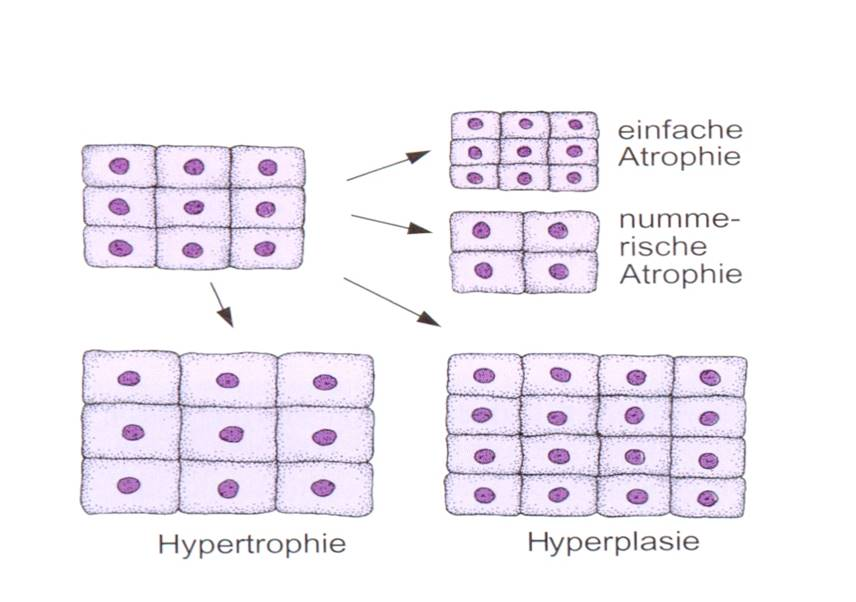
\includegraphics[scale=0.7]{Picture1.jpg}
	\end{center}
\pagebreak
\subsubsection{quantitative Wachstumsstörungen}
	\begin{itemize}
		\item meist reversibel
		\item \textbf{Atrophie = Verminderung des Zellwachstums} (Atropie - Rückbildung)
			\begin{itemize}
				\item \textbf{Verkleinerung eines primär normal entwickelten und normal großen Gewebes bzw. Organs}
				\item \textbf{Überwiegen der katabolen über die anabolen Stoffwechselvorgänge}
					\begin{itemize}
						\item \textbf{einfache Atrophie: Zellverkleinerung}
						\item \textbf{numerische Atrophie: Verminderung der Zellzahl}
					\end{itemize}
				\item \textbf{physiologische Atrophie}
					\begin{itemize}
						\item \textbf{im Rahmen normaler physiologischer Entwicklungsprozesse}
						\item Unmittelbar nach der Geburt - Nabelschnurgefäße
						\item Gebärmutter nach der Geburt - Bildet sich wieder zurück
						\item Geschlechtsorgane bilden sich im Alter zurück
						\item Thymosdrüse - aktiv in der Kindheit und Heranwachsen - bilden T-Lymphozyten
					\end{itemize}
				\item \textbf{pathologische Atrophie}
					\begin{itemize}
						\item \textbf{im Rahmen krankhafter Ereignisse, Überwiegen der katabolen Prozesse}
					\end{itemize}
			\end{itemize}
%\pagebreak
		\item \textbf{lokale Atrophien}
			\begin{itemize}
				\item \textbf{auf ein Organ oder einen Gewebsabschnitt beschränkt}
					\begin{itemize}
						\item \textbf{Inaktivitätsatrophie}
							\begin{itemize}
								\item weniger funktionelle Beanspruchung $\rightarrow$ Atrophie
								\item Gips führ zur Rückbildung der Muskeln
							\end{itemize}
						\item \textbf{vaskuläre Atrophie $\rightarrow$ Ischämie}
							\begin{itemize}
								\item Atrophie der Haut um Unterschenkel - Venöser Abtransport schlecht durch Krampfadern $\rightarrow$ Atrophieren der Haut - Schlechte Wundheilung, dünne Haut, leicht verletzbar
							\end{itemize}
						\item \textbf{mechanische Druckatrophie $\rightarrow$ Kompression}
						\item \textbf{neurogene Atrophie (fehlende Innervation)}
						\item \textbf{Erschöpfungsatrophie}
							\begin{itemize}
								\item Mehrforderung - Organ wächst durch langfristige Überforderung $\rightarrow$ Atrophie
							\end{itemize}
						\item \textbf{endokrine Atrophie (mangelnder hormoneller Stimulus)}
							\begin{itemize}
								\item männlicher Alkoholiker, Leber kann Östrogen nicht mehr abbauen, Östrogenüberschuss $\rightarrow$ Hodenatrophie, Brustdrüsenwachstum
							\end{itemize}
						\item \textbf{genetisch bedingte Atrophie}
					\end{itemize}
				\item \textbf{generalisierte Atrophien}
					\begin{itemize}
						\item \textbf{den gesamten Körper betreffend}
							\begin{itemize}
								\item \textbf{senile Atrophie}, alles was in Verwendung ist wird weniger atrophieren
								\item \textbf{Hungeratrophie}, Fettgewebe, Muskeln sind atrophiert, allerdings nicht das Gehirn, Magersucht
								\item \textbf{Kachexie}, Atrophie des gesamten Körpers, beispielsweise durch schwere Erkrankung, fortgeschrittene Tuberkulose
							\end{itemize}
				\end{itemize}
			\end{itemize}
		\item \textbf{angeborene Störungen mit Hemmung des Wachstums}
			\begin{itemize}
				\item \textbf{Agenesie: gesamte Organanlage fehlt}
				\item \textbf{Aplasie: Organentwicklung fand nicht statt}
				\item \textbf{Hypoplasie: Organentwicklung kam vorzeitig zum Stillstand (Unterentwicklung)}
			\end{itemize}
\pagebreak
		\item \textbf{Hypertrophie} (reine Zellvergrößerung)
			\begin{itemize}
				\item \textbf{Organvergrößerung durch Zellvergrößerung ohne Zellvermehrung}
				\item \textbf{Steigerung der Leistungsfähigkeit, jedoch Verminderung der Reserve}
					\begin{itemize}
						\item \textbf{Arbeitshypertrophie (vermehrte Arbeitsbelastung)} (Muskelypertrophie - Skelettmuskulatur
						\item \textbf{kompensatorische Hypertrophie}
					\end{itemize}
				\item zuviel Wachstum, mehr Leistung gefordert $\rightarrow$ Wachstum nur bis zu gewissem Grad mit Versorgung möglich
				\item Zurückbildung wenn die Leistungsforderung nachlässt
				\item Herz - Sportlerherz
			\end{itemize}
		\item \textbf{Hyperplasie} (Vermehrung der Zellanzahl)
			\begin{itemize}
				\item \textbf{Organvergrößerung durch Zellvermehrung}
				\item \textbf{regeneratorische Hyperplasie}
					\begin{itemize}
						\item \textbf{Reaktion auf Gewebeschädigung mit überschießender Regeneration / Reparation}
							\begin{itemize}
								\item Narbengewebe bei bleibender Belastung unelastisch, Problem wenn dies über ein Gelenk verläuft
							\end{itemize}
					\end{itemize}
				\item \textbf{Hyperplasien infolge endokriner Störungen}
					\begin{itemize}
						\item \textbf{vermehrter Hormonstimulus}
							\begin{itemize}
								\item Prostatahyperplasie - relative Vermehrung der weiblichen Geschlechtshormone - Außenteile der Prostata hyperplasierend $\rightarrow$ Probleme in der Harnentleerung (Einengung der Harnröhre)
							\end{itemize}
						\item \textbf{z.B. Hyperplasie der Prostata, Hyperplasie der Schilddrüse}
						\item Hyperplasie der Schilddrüse - Kropf bei Jodmangel 
					\end{itemize}
			\end{itemize}
	\end{itemize}

\subsubsection{qualitative Wachstumsstörungen}
	\begin{itemize}
		\item \textbf{Metaplasie}
			\begin{itemize}
				\item \textbf{Ersatz eines ausdifferenzierten} (robusteren) \textbf{Gewebes durch anderes hochdifferenziertes Gewebe}
				\item Raucherlunge - Flimmerepidel $\rightarrow$ Palltenepidel aufgrund von Belastung 
			\end{itemize}
		\item \textbf{Dysplasie}
			\begin{itemize}
				\item \textbf{meist noch reversible Veränderungen von Zellen durch atypische Regeneration und Verlust der Differenzierung fließender Übergang zur (irreversiblen) Anaplasie}
				\item Formveränderung, Größenveränderung der Zellen
			\end{itemize}
		\item \textbf{Anaplasie}
			\begin{itemize}
				\item \textbf{irreversible Entdifferenzierung der Zellen und Gewebe mit Verlust der geweblichen Struktur und der Formbesonderheiten der Zellen = Malignität}
				\item Bösartigkeit von Gewebe
			\end{itemize}
	\end{itemize}
	\section{Tumorlehre}
	\subsection{Grundlagen}
		\begin{itemize}
			\item \textbf{Tumor} (lat) \textbf{("onkos")} (gr) \textbf{= Schwellung = Volumenzunahme}
			\item \textbf{synonym: Neoplasma} (Neoplasie) \textbf{("Neubildung"), Blastom}
				\begin{itemize}
					\item \textbf{Neubildung körpereigenen Gewebes mit autonomer Wachstumstendenz, die jene eines normalen Gewebes weit übersteigt}
					\item \textbf{Wachstum ist unkontrolliert und überschießend, auf Kosten der gesunden Zellen (Nährstoffentzug!)} Geht weiter, auch wenn es keine Ursache mehr dafür gibt.
					\item \textbf{Wachstum wird auch nach Wegfall der auslösenden Ursache nicht eingestellt}
						\begin{itemize}
							\item \textbf{vgl. Hypertrophie/-plasie: Wachstum vom auslösenden Reiz abhängig, reversibel}
						\end{itemize}
				\end{itemize}
			\item \textbf{Dignität: es gibt gutartige (benigne) und bösartige (maligne) Tumore}
				\begin{center}
					\begin{tabular}{|rl|}
						\hline
						\textbf{benigne Tumore} & \textbf{maligne Tumore} \\
						\hline
						\multicolumn{2}{|c|}{\textbf{Wachstum}} \\ 
						langsam & rasch \\ 
						scharf begrenzt (Kapsel) & unscharf begrenzt \\ 
						expansiv, verdrängend & infiltrativ, eindringend \\
						komprimierend & destruierend \\
						eher verschieblich & nicht verschieblich \\
						\multicolumn{2}{|c|}{\textbf{Zellen}} \\
						keine Zellatypien & Zellatypien (Analplasie) \\
						differenziert & undifferenziert \\
						reif & \pbox{20cm}{unreif (nicht höher ausgebildet,\\ keine Feinheiten in der Ausbildung)} \\
						\multicolumn{2}{|c|}{\textbf{Metastasen}} \\
						keine Metastasen & \pbox{20cm}{bildet Metastasen: Streuung,\\Aussiedeln an anderen Stellen im Körper} \\
						\multicolumn{2}{|c|}{\textbf{Verlauf}} \\
						geringe Allgemeinstörung & starke Allgemeinstörung \\
						\pbox{20cm}{wenig Rezidive: kein Erneutes\\ Wiederauftreten nach Heilung} & oft Rezidive \\
						meist keine direkte Lebensgefahr & meist hohe Lebensgefahr\\
						\hline
					\end{tabular}
				\end{center}
			\item Es ist kenie klare Abgrenzung und Unterscheidung möglich, der Übergang ist fließend.
		\end{itemize}
	\subsection{borderline lesions (=semimaligne Tumore)}
		\begin{itemize}
			\item \textbf{wachsen bösartig (lokal infiltrativ und destruierend)}
			\item \textbf{hochgradige Rezidivneigung}
			\item \textbf{metastasierend, jedoch sehr selten und sehr spät}
		\end{itemize}
	\subsection{Präkanzerosen}
		\begin{itemize}
			\item "vor dem Krebs"
			\item \textbf{Gewebsveränderungen mit erhöhtem Risiko der malignen Entartung}
			\item \textbf{fakultative Präkanzerose: Entartungsrisiko $<$ 20\%, Dauer $>$ 5 Jahre} (Colotis ulcerosa - Darm)
			\item \textbf{obligate Präkanzerose: Entartungsrisiko $>$ 20\%, Dauer $<$ 5 Jahre}
				\begin{itemize}
					\item hohes Risiko
					\item Durch Gendefekt in Familien
					\item starkes Polypenwachstum (gestielt - Adenom) im Dickdarm mit großem Entartungsrisiko $\rightarrow$ Entfernung des Dickdarmstückes
					\item[$\rightarrow$] Stuhl nicht mehr eingedickt, künstlicher Darmausgang, hoher Leidensdruck
					\item familiäre Ademomatose
				\end{itemize}
		\end{itemize}
\pagebreak
	\subsection{Metastasen}
		\begin{itemize}
			\item \textbf{Absiedlungen (Tochtergeschwülste) vom Primärtumor (Muttergeschwulst) über}
				\begin{itemize}
					\item \textbf{den Lymphweg (lymphogen)}
						\begin{itemize}
							\item \textbf{regionale Lymphknoten - weitere Lymphknotengruppen - über den Ductus thoracicus in das Blutgefäßsystem}
								\begin{itemize}
									\item Normalerwise bekämpft das Immunsystem alleinschwimmende Zellen
									\item Sentinallymphnode - es wird der Fluss der Lymphe analysiert und die jeweiligen Lymphknoten werden dann ausgeräumt und von Tumorzellen befreit.
									\item Tumorzelle tarnt sich - Lymphe gefüllt mit Abwehrzellen
								\end{itemize}
						\end{itemize}
					\item \textbf{den Blutweg (hämatogen)}
						\begin{itemize}
							\item \textbf{arterieller Typ}
								\begin{itemize}
									\item Primärtumor Lunge, Verschleppung Ateriell im Körper
									\item Tumorzellen nicht gern in stark durchströmten Gefäßen $\rightarrow$ Kapillargewebe + Ansiedelung (Lunge) - (Kein Tumor im Herz)
								\end{itemize}
							\item \textbf{Holvenen Typ}
							\item \textbf{Pfortadertyp}
								\begin{itemize}
									\item Dickdarmkrebs $\rightarrow$ Leber (primär metastasierend) $\rightarrow$ Lunge, hämatogener Weg ist anatomisch vorgegeben
								\end{itemize}
							\item \textbf{vertebraler Typ}
								\begin{itemize}
									\item Tumorzellen aus Prostata in Lendenwirbel. (Ebenfalls Rückschluss von der Metastase auf den Primärtumor möglich)
								\end{itemize}
						\end{itemize}
					\item \textbf{innerhalb der Körperhölen (Absiedelung an Pleura, Peritoneum}
						\begin{itemize}
							\item im Torax - Ausbreitung flächig über die Pleura
						\end{itemize}
					\item \textbf{kanalikulär}
						\begin{itemize}
							\item Nutzung der Tumorzelle von bestehenden Kanälen (Magen/Darm)
						\end{itemize}
					\item \textbf{Knochenmetastasen (indifferent, osteoblastisch, osteoklastisch)}
						\begin{itemize}
							\item Metastasen als Fremdgewebe identifizierbar $\rightarrow$ Ursprung des Tumors diagnostizierbar
							\item osteoblastisch - Verdichten der Knochen - lässt Rückschlüsse auf Primärtumor zu.
						\end{itemize}
				\end{itemize}
			\item Zellen passen jeweils auf den Verband auf. Sobald sich eine daraus löst, wird das Immunsystem aktiviert. Auch werden defekte und fehlerhafte Zellen normalerweise ausgesondert. Beim Tumor erkennt das Immunsystem diesen Fehlerfall nicht (Möglichkeit der Markierung von Tumorzellen)
			\item Bewegung erleichtert das Lösen von Metastasen vom Primärtumor, ebenfalls ist eine iatrogene Manipulation möglich, Operation im Tumorgebiet.
			\item Terrainfaktor: bestimmte Tumore metastasieren in bestimmte Organe - die Tumorzellen werden dort nicht als fremd erkannt.
			\item Frühmetastasen / Spätmetastasen (nach zB. 20 Jahren vermehrt sich die Tumorzelle im Zielgebiet)
			\item Faktoren welche die Metastasierung begünstigen:
				\begin{itemize}
					\item starkes Primärtumorwachstum
					\item viele Nekrosen im Tumorgebiet
					\item Gefäßreichtum eines Tumors
					\item geringer Zusammenhalt des Tumorgewebes
				\end{itemize}
			\item Auch wenn sie sich in Fremdgewebe ansiedeln, müsste das Immunsystem anspringen. Die Tumorzellen adaptieren sich, oder sind autonom um die Kommunikation (Energiehaushalt) zu Nachbarzellen zu verhindern. Tumorentwicklung hängt mit Abwehrschwäche zusammen.
		\end{itemize}
	\subsection{Tumorrezidiv}
		\begin{itemize}
			\item gleicher Tumor an gleicher Stelle
			\item \textbf{entsteht aus liegen gebliebenen Zellen eines unvollständig entfernten Primärtumors}
			\item Tumorzellen schlummern in Lymphspalten (kann Jahre dauern), die Wahrscheinlichkeit ist äquivalent zum Alter des Ersttumors
		\end{itemize}
	\subsection{5-Jahres-Heilungsrate / 5-Jahres-Überlebensrate}
		\begin{itemize}
			\item als Durchschnittswert zu verwenden
			\item Statistisch 5-Jahres-Überlebensrate nur sehr gering, weil es sich hier um schwere Tumore handelt (Lungenkrebs), zu späte Diagnose häufig
			\item \textbf{fünf Jahre nach der Behandlung eines malignen Tumors weder ein Rezidiv noch Metastasen nachweisbar (= Behandlungserfolg) / überlebt}
			\item Nur begrenzt aussagekräftig, auch andere Krankheitsfälle die nichts mit dem Tumor zu tun haben, werden aufgenommen.
		\end{itemize}
	\subsection{Tumorbeurteilung}
		\begin{itemize}
			\item \textbf{typing}
			\item \textbf{staging}
			\item \textbf{grading}
		\end{itemize}
	\subsection{typing (Tumornomenklatur)}
		\begin{itemize}
			\item \textbf{Benennung der Tumore: Endung  "-om"}
			\item \textbf{Bezeichnung nach der Bauart bzw. dem Muttergewebe} (Mutter und Tochtergeschwulst)
				\begin{itemize}
					\item \textbf{Drüsengewebe} (Adeno-om)
					\item \textbf{Bindegewebe} (Fibro-om)
					\item \textbf{Fettgewebe} (Lipom)
					\item \textbf{Muskelgewebe} (Myom)
					\item \textbf{Knorpelgewebe} (Chondrom)
					\item \textbf{Knochengewebe} (Osteom)
					\item \textbf{Blutgefäße} (Ham Angion)
				\end{itemize}
			\item \textbf{Mischtumore: Tumoren mit sowohl epithelialen als auch mesenchymalen Anteilen (z.B. Fibroadenom)} (Deckgewebe, Haut Schleimhaut, Drüsengewebe)
			\item \textbf{maligner epithelialer Tumor: Carcinom} (organspezifisches Gewebe (Muskeln, Knorpel, Blutgefäße, $\dots$)
				\begin{itemize}
					\item Großteil der Tumore sind carcinome Tumore, Epithelgewebe natürlich teilungsfreudig, mechanische Einflüsse, große Flächen
				\end{itemize}
			\item \textbf{maligner mesenchymaler Tumor: Sarkom}
			\item \textbf{Tumore des lymphatischen Systems:}
				\begin{itemize}
					\item \textbf{maligne Lymphome}
						\begin{itemize}
							\item weiße Blutzellen (maligne Leukosen / Entartung $\rightarrow$ Leukämie)
						\end{itemize}
				\end{itemize}
			\item \textbf{Tumore des blutbildenden Systems bzw.Knochenmark:}
				\begin{itemize}
					\item \textbf{maligne Leukosen bzw. Leukämie}
				\end{itemize}
			\item \textbf{Tumore des Nervensystems:}
				\begin{itemize}
					\item \textbf{Gehirnzwischensubstanz (Gliazellen)}
					\item \textbf{Hirnhaut (Meningen)}
					\item \textbf{periphere Nerven (Schwann'sche Zellen)}
				\end{itemize}
			\item \textbf{Tumore des pigmentbildenden Systems}
				\begin{itemize}
					\item \textbf{Nävus} (gutartig, Muttermal)
					\item \textbf{malignes Melanom} (bösartig)
				\end{itemize}
		\end{itemize}
	\subsection{staging: Tumorstadien - Klassifizierung nach dem TNM-System:}
		\begin{itemize}
			\item \textbf{Feststellung der Ausbreitung des Tumorgewebes}
						\begin{itemize}
							\item \textbf{am primären Entstehungsort (Primärtumor = T)}(1-4)
							\item \textbf{Befall der Lymphknoten (Nodulus = N)}(1-3)
							\item \textbf{entferntere Organe (Metastasen = M)}(0-1)
						\end{itemize}
			\item \textbf{wichtig für Therapiewahl und Prognose!}
			\item \textbf{pTNM-Klassifizierung = postoperativ = aussagekräftiger!} (Post-OP Parafinschnitt genauer!)
		\end{itemize}
	\subsection{grading: Beurteilung der Malignität}
		\begin{itemize}
			\item Grad der Naplase, Bsp.: hohe Mitose
			\item \textbf{Grundlage für weitere Therapie und Prognose}
				\begin{itemize}
					\item \textbf{3 (4) Malignitätsgrade}
						\begin{itemize}
							\item \textbf{G1, niedrigste Malignität}
							\item \textbf{G3, oder 4,  höchste Malignität}
						\end{itemize}
					\item \textbf{Kriterien}
						\begin{itemize}
							\item \textbf{gewebliche Entdifferenzierung}
							\item \textbf{Grad der Anaplasie}
							\item \textbf{Wachstumstendenz}
							\item \textbf{(Verhalten zum umliegenden Gewebe)}
						\end{itemize}
				\end{itemize}
		\end{itemize}
	\subsection{Tumorhäufigkeit}
		\begin{itemize}
			\item \textbf{Frauen}
				\begin{itemize}
					\item \textbf{Inzidenz} (=Neuauftreten)
						\begin{itemize}
							\item Brist
							\item Darm
							\item Gebärmutter
							\item Eierstöcke
							\item Magen
							\item Lunge
						\end{itemize}
					\item \textbf{Mortalität}
						\begin{itemize}
							\item Brust
							\item Darm
							\item Lungen
						\end{itemize}
				\end{itemize}
			\item \textbf{Männer}
				\begin{itemize}
					\item \textbf{Inzidenz}
						\begin{itemize}
							\item Prostata
							\item Darm
							\item Lunge
						\end{itemize}
					\item \textbf{Mortalität}
						\begin{itemize}
							\item Lungenkrebs
							\item Darm
							\item Prostata
						\end{itemize}
				\end{itemize}
			\item Durchbruch noch nicht gelungen. Man versteht die Ursachen noch lange nicht.
		\end{itemize}
	\subsection{Folgen maligner Neoplasmen:}
		\begin{itemize}
			\item \textbf{lokal}
				\begin{itemize}
					\item \textbf{Organfunktionsstörungen}
					\item \textbf{Stenosen oder Verschluss von Hohlorganen}
						\begin{itemize}
							\item Stenose - Einengung von Öffnungen
							\item Nekrose - Zerstörung von Gewebe
							\item brauchen Platz und Energie, sind parasitär
						\end{itemize}
					\item \textbf{Tumornekrosen}
				\end{itemize}
			\item \textbf{allgemein:}
				\begin{itemize}
					\item \textbf{Tumorkachexie}
					\item \textbf{Fieber}
					\item \textbf{Tumoranämie}
						\begin{itemize}
							\item Zerstörung von Blutzellen (weiß, rot) $\rightarrow$ Depression, Infektanfälligkeit
						\end{itemize}
					\item \textbf{Infektanfälligkeit und herabgesetzte Immunabwehr}
					\item \textbf{endokrine Effekte bei endokrin-aktiven Tumoren}
						\begin{itemize}
							\item hormonelle Aktivität, Lungenkrebs erhöhen Kalziumspiegel im Blut
						\end{itemize}
					\item \textbf{paraneoplastische Syndrome}
				\end{itemize}
		\end{itemize}
	\subsection{Todesursachen bei malignen Tumoren}
		\begin{itemize}
			\item \textbf{Zerstörung lebenswichtiger Organe}
			\item \textbf{akute oder chronische Blutungen}
			\item \textbf{Verschluss wichtiger Hohlorgane}
			\item \textbf{Infektion}
			\item \textbf{Metastasierung in lebenswichtige Organe}
			\item \textbf{Herzversagen}
				\begin{itemize}
					\item zusätzliches Gewebe benötigt zusätzliche Durchblutung
				\end{itemize}
			\item \textbf{Tumorkachexie}
				\begin{itemize}
					\item auf Kosten des gesunden Gewebes $\rightarrow$ Ausgezehrtheit
				\end{itemize}
		\end{itemize}
\pagebreak
	\subsection{Ätiologie maligner Neoplasmen}
		\begin{itemize}
			\item \textbf{Krebsentstehung: Zusammenwirken verschiedener krebserregender Faktoren}
			\item \textbf{endogene Ursachen}
				\begin{itemize}
					\item \textbf{genetische Faktoren}
						\begin{itemize}
							\item ~5\% 
							\item Bsp1.: familiäre Dickdarm-Adenomatose = fam. Polyposis
								\begin{itemize}
									\item Polypen: gutartige Tumore, aus denen mit d. Zeit bösartige entstehen können, treten im Alter einzeln auf, werden häufig Kontrolliert und ggf. entfernt
									\item bei Polyposis: hunderte mit hohem Entartungsrisiko, in kurzer Zeit, auch in jungen Jahren! Engmaschige Kontrollen, ggf. operative Entfernung der betroffenen Dickdarm-Teile (muss zu viel entfernt werden, kann nicht mehr ausreichend eingedickt werden $\rightarrow$ künstlicher Ausgang = Stoma) 
									\item Fehlen eines Tumor-Suppressor Gens (erstes entdecktes Tumor-Suppressor-Gen: p53Gen)
								\end{itemize}
							\item Bsp2.: Gendefekt-verursachtes Mamma-Karzinom (sehr selten): sehr hohes Risiko, Angebot der präventiven Brust-Amputation
						\end{itemize}
					\item  \textbf{hormonelle Faktoren} \\
						zB.: Prostata Carcinom (Details folgen)						
					\item	\textbf{chronische Gewebereizung} \\
						Chronisch gereiztes Gewebe hat höheres Karzinom Risiko\\
						zB.: chronische Entzündung, schlecht sitzende Implantate 
				\end{itemize}
			\item \textbf{exogene Ursachen}
				\begin{itemize}
					\item \textbf{chemische Faktoren}
						\begin{itemize}
							\item häufigste Ursache
							\item bei geringer Dosis kann es durchaus lange dauern bis Auftreten, aber: Dosisakkumulation!
							\item Beispiele für chemische Verbindungen
								\begin{itemize}
									\item Benzidin, Anilin $\rightarrow$ Harnblasencarcinom
									\item Benzpyren, polyzyklische Wasserstoffe $\rightarrow$ Hautcarcinom
									\item versch. Substanzen $\rightarrow$ Lebercarcinom
										(zB Schimmelpilz im Getreide $\rightarrow$ Aflatoxin) 
									\item Arsen/Chrom Verbindungen
									\item Asbest, Nickel \& Holzstaub $\rightarrow$ Lungen und Nasennebenhöhlen
									\item Asbest $\rightarrow$ Pleuramesotheliom
									\item Nitrosamine, in gepökeltem/verbranntem Fleisch $\rightarrow$ Magen\\
										(daher in Tirol \& Vorarlberg höher wegen Speck, Japan durch geräucherten gepökeltem Fisch)
									\item Tabak $\rightarrow$ Mundhöhle, Lunge, Kehlkopf, Speiseröhre (meist Alkohol+Nikotin), Harnblase, Lippencarcinom (betrifft auch Zigarrenraucher - ohne Inhalation)
									\item Hormone:\\
										\mbox{}\quad ' Androgene: doping – Leber\\
										\mbox{}\quad ' Pille - geringe Erhöhung gutartiger Lebertumore, aber deutliche Senkung d. \\
										\mbox{}\quad\:  Ovarialencarzinome
								\end{itemize}
						\end{itemize}
					\item \textbf{physikalische Faktoren}
						\begin{itemize}
							\item Radioaktive Strahlung
								\begin{itemize}
									\item[$\rightarrow$] Plattenepidelkarz. an Händen durch ungeschützten, direkten Kontakt (z.B. erste Radiologie-Forscher, Hiroshima, Nagasaki, Tschernobyl: DNA-Schädigung $\rightarrow$ Leukämien, Schildrüsencarcinom)
								\end{itemize}
							\item UV-Strahlung: DNA-Schädigung
								\begin{itemize}
									\item[$\rightarrow$] Plattenepidelcarzinom, Melanom (maligner Hauttumor), Basaliom (Haut "merkt" sich Schädigung, muss nach UV-Einstrahlung Reparaturmaßnahmen durchführen. $\rightarrow$ bei zu viel UV-Einwirkung überfordert)
									\item Melanom: genetische Veranlagung, eventuell Viren u.a. unbekannte Einflüsse. Auch bei jungen Erwachsenen möglich
								\end{itemize}		  
						\end{itemize}
\pagebreak	
					\item \textbf{infektiöse Faktoren} (onkogene Viren, selten Alleinauslösende Faktoren)
						\begin{itemize}
							\item Humanes Papillomavirus: Warzen an Haut u. Genitalien, deutlich erhöhtes 
								\begin{itemize}
									\item Cervixkarzinomrisiko (Impfung gegen die häufigsten Arten, kostspielig!)
									\item STD! durch oralen Verkehr: Larynxkarzinomrisiko $\dagger$
								\end{itemize}
							\item Herpes-Simplex-Virus (HSV) \emph{Typ2}: genitaler Herpes $\rightarrow$ Cervixkarzinomrisiko $\dagger$
							\item Epstein-Barr-Virus: Preiffer'sches Drüsenfieber = Mononukleose
								\begin{itemize}
									\item engl. umgs. kissing disease
									\item (sichtbare) Schwellung der Hals-Lymphknoten
									\item meist komplikationslose Erkrankung i.d. Pubertät, aber: erhöhtes Risiko für maligne Lymphome
								\end{itemize}
						\end{itemize}
					\item \textbf{Ernährung}
						\begin{itemize}
							\item Nitrosamine, Ballaststoffe, tierische Fette? $\dots$
						\end{itemize}
				\end{itemize}
		\end{itemize}
	\subsection{Onkogenese (Karziogenese)}
		\begin{itemize}
			\item \textbf{immunologische Reaktion des Wirtsorganismus}
				\begin{itemize}
					\item Immun-Überwachungs-Theorie: fehlende immunologische Reaktion des Wirtsorganismus auf entartete Tumorzellen
				\end{itemize}
			\item \textbf{Tumorwachstum: Zellkommunikationsstörung}
				\begin{itemize}
					\item Zellkommunikationsstörung $\rightarrow$ Tumorwachstum
				\end{itemize}
			\item \textbf{Tumor-Angiogenese-Faktor: ausreichende Blutversorgung ist für das Tumorwachstum essentiell}
			\item \textbf{Invasion und Metastatsierung: verminderter interzellurärer Zusammenhalt}\\
				zB. Tarnung als Thrombus
		\end{itemize}
	\subsection{Diagnostik: Tumormarker}
		\begin{itemize}
			\item \textbf{im Blut messbare Substanzen, die mit malignem
				Tumorgewebe korrelieren \emph{können}}
			\item aber: \textbf{nicht tumorspezifisch, nicht organspezifisch}
			\item \textbf{Nachweis teilweise bis zu Grenzwert normal}
			\item \textbf{daher v.a. für postoperative Verlaufskontrolle}\\
				Vergleich mit pre-OP Wert
			\item \textbf{Beispiele:}
				\begin{itemize}
					\item \textbf{AFP} Alpha Feto Protein, \textbf{CEA} Carcino Enbryonales Antigen:
						\begin{itemize}
							\item Bei Embryos vorhanden, gehen m.d.Z. verloren, bilden sich bei Erkrankung neu
							\item Bsp: Dickdarmcarzinom
						\end{itemize}
					\item \textbf{HCG} Humanes Choriongonadotropin (von Tumorzellen erzeugte Hormone)
						\begin{itemize}
							\item wird auch an Beginn der Schwangerschaft gebildet (Schwangerschaftstest!)
							\item gut verwertbar beim Mann $\rightarrow$ Hodentumor
						\end{itemize}
					\item \textbf{Calcitonin}: Kann mit Schilddrüsenkarzinom korrelieren
					\item Enzyme: \textbf{PSA} Enzyme: Prostata Spezifisches Antigen, \textbf{PAP} Prostatic Acid Phosphatase (Indikator erst ab physiologischem Schwellwert)
				\end{itemize}
		\end{itemize}
	\subsection{Behandlung}
		\begin{itemize}
			\item \textbf{Operation}
			\item \textbf{Radiotherapie}
				\begin{itemize}
					\item \textbf{Zelltod duch ionisierende Stahlung, präoperative und/oder postoperative Bestrahlung}
					\item auch pre-OP, verkleinert den Tumor, zerstört besonders aktive Zellen, verringert OP-bedingtes Streuungsrisiko
					\item Stahlen und Chemotherapie zerstört alles teilungsfreudige Gewebe $\rightarrow$ enorme Nebenwirkungen
					\item keine neuen Blutzellen, Schleimhäute, Haarausfall, Hautschäden, Zerfall vieler Zellen
					\item verursacht Gewebeschäden - gesundes Gewebe wird verletzt
				\end{itemize}					
			\item \textbf{Chemotherapie mit Zytostatika}
				\begin{itemize}
					\item Gewebetoxisch - Zerstören die Wände von kleinen Venen
				\end{itemize}
		\end{itemize}
	\subsection{neuere Methoden}
		\begin{itemize}
			\item \textbf{monoklonale Antikörper}
				\begin{itemize}
				\item weist der Tumor Antigenkörper auf, kann man Antikörper geben, die Tumorzellen zerstören sollen
				\end{itemize}
			\item \textbf{dendritische Zelltherapie}
			\item \textbf{Hyperthermie}
			\item \textbf{Neutronenstrahlung}
			\item \textbf{$\dots$}
		\end{itemize}
	\subsection{Nebenwirkungen}
			\begin{itemize}
				\item auch gesunde Zellen in Teilung werden vorübergehend zerstört. Vor allem
					\begin{itemize}
						\item Haut- und Schleimhautzellen, Haare $\rightarrow$ Haarausfall
						\item Blutzellen
							\begin{itemize}
								\item[$\rightarrow$] Erythrozytenmangel $\rightarrow$ Anämie (Schwäche, depressive Verstimmung, …)
								\item[$\rightarrow$] Leukozytenmangel $\rightarrow$ Schwächung d. Immunsystems $\rightarrow$ mangelnde Abwehr, Infektanfälligkeit
							\end{itemize}
					\end{itemize} 
				\item \textbf{sekundäre Neoplasien}
					\begin{itemize}
						\item ionisierende Strahlung ist cancerogen (Bsp. 10-20 Jahre später)
					\end{itemize}
				\item \textbf{Knochenmarkschädigung}
				\item \textbf{gastrointestinale Nebenwirkungen}
				\item \textbf{Haarausfall (Alopezie)}
				\item \textbf{Hyperpigmentierung der Haut}
				\item \textbf{Fieber, Schüttelfrost, depressive Verstimmung}
				\item \textbf{Organschäden (Leber, Niere, Lunge, Herz, Muskulatur, Nerven)}
				\item \textbf{lokale Gewebstoxizität}			
			\end{itemize}
	
\pagebreak
\subsection{einzelne Tumorbeispiele}
	\begin{itemize}
		\item \textbf{Malignes Melanom}
			\begin{itemize}
			\item Abgrenzung zum benignen Naevus (Muttermal)\\
				ABCD(E)-Regel
					\begin{itemize}
						\item Asymmetrie
						\item Begrenzung
						\item Colour
						\item Durchmesser
						\item (Erhaben)
					\end{itemize}
			\end{itemize}
		\item \textbf{Basaliom}
			\begin{itemize}
				\item "semimaligne" = borderline, lokal malignes Wachstum aber keine Metastasierung!
			\end{itemize}
		\item \textbf{Leukämien}
			\begin{itemize}
				\item Einteilung
					\begin{itemize}					
						\item akute Leukämie
							\begin{itemize}
								\item 90\% Leukämien im Kindesalter
								\item myeloische ($\rightarrow$ akute meloische Leukämie)
								\item lymphatische ($\rightarrow$ akute lymphatische Leukämie)
							\end{itemize}
						\item chronische Leukämie
							\begin{itemize}
								\item myeloische ($\rightarrow$ chronische myeloische Leukämie)
								\item lymphatische ($\rightarrow$ chronische lymphatische Leukämie)
							\end{itemize}
						\item[$\rightarrow$] Mangel an Erythrozyten = Anämie
						\item[$\rightarrow$] Mangel an Trombozyten $\rightarrow$ Blutgerinnungsproblem, Spontanblutungen
						\item[$\rightarrow$] Mangel an Leukozyten $\rightarrow$ Abwehrschwäche, Infektanfälligkeit
					\end{itemize}
			\end{itemize}
		\item \textbf{maligne Lymphome}
			\begin{itemize}
				\item M(orbus)-Hodgkin-Lymphom
					\begin{itemize}
						\item geht von B-Lympozyten aus
						\item Symptome
							\begin{itemize}
								\item Nachtschweiß, Gewichtsverlust, evtl. Fieber
								\item erhöhte BSG, Blutsenkungsgeschwindigkeit (später mehr)
								\item manchmal Schmerzen/Juckreiz nach Alkoholkonsum
							\end{itemize}
						\item Staging:
							\begin{itemize}
								\item Eine, zwei, mehrere Knoten befallen
								\item Behandlung: Strahlen \& Chemo
							\end{itemize}
						\item Prognose:
							\begin{itemize}
								\item bei Früherkennung 70\% Überlebensrate
							\end{itemize}
					\end{itemize}
				\item Non-Hodgkin-Lymphom
			\end{itemize}		
		\item \textbf{Hodencarcinom}
			\begin{itemize}
				\item Altersgipfel: 20-30
				\item überwiegend von Keimzellen ausgehend $\rightarrow$ Keimzellentumore (häufigster maligner Tumor bei jungen Männern)
				\item Ätiologie: risikoerhöhend: Hoden zum Zeitpunkt der Geburt nicht im Skrotum (noch in Bauchhöhle)
			\end{itemize}
		\item \textbf{Prostatacarcinom}
			\begin{itemize}
				\item überwiegend ältere ältere Männer
				\item durch Abfall von Testosteron relativer Anstieg von Östrogen $\rightarrow$ Wachstumsstimulus für Prostata
				\item Therapie:
					\begin{itemize}
						\item OP (möglichst Nerven-schonend! aber: höheres Risiko, nicht alle Carcinom-Anteile zu entfernen!)
						\item Hormontherapie: anti-androgen (Nebenwirkung: „Verweiblichung“ $\rightarrow$ z.B. Brustdrüsenwachstum)
					\end{itemize}
			\end{itemize}
		\pagebreak
		\item \textbf{Mammacarcinom}
			\begin{itemize}
				\item Insidenz nimmt stetig zu, zZt. jede 8. Frau
				\item Lokalisation meist obere Hälfte
				\item Risikofaktoren
					\begin{itemize}
						\item genetische Veranlagung
						\item Östrogene
							\begin{itemize}
								\item frühe Menarche (erste Regelblutung)
								\item späte Monopause
								\item Östrogentherapie i.d. Menopause
								\item Keine Schwangerschaften (Schwangerschaft+Stillzeit unterbricht Zyklus)
								\item Adipositas
							\end{itemize}
					\end{itemize}
				\item mit dem Alter deutlich Ansteigend nach 50
				\item gute Prognose
				\item Behandlung
					\begin{itemize}
						\item Operation
							\begin{itemize}
								\item Entfernung von Lymphknoten in der Achsel, wird kaum noch durchgeführt
							\end{itemize}
						\item kosmetische Restauration
					\end{itemize}
			\end{itemize}
		\item \textbf{Cervixcarcinom}
		\item \textbf{Coloncarcinom}
			\begin{itemize}
				\item Insidenz nimmt stetig zu, vermutlich auf Grund von Lebensweise
				\item möglicherweise Ernärung und Genetik Ursachen\\
					(cancerogene Lebensmittel bleiben länger im Colon durch balaststoffarme Ernärung)
				\item 90\% entwickeln sich aus malignen Polypen\\
					  Vorsorgliche Spiegelung im höheren Alter, Entfernung und Analyse der Polypen (Poloskopie)
				\item Therapie
					\begin{itemize}
						\item Im Krankheitsfall Chemotherapie und Operation, nicht aber Bestrahlung (Beschädigung der umliegenden Organe)
					\end{itemize}
				\item Metastasen $\rightarrow$ Leber $\rightarrow$ Lunge 
				\item 90\% Überlebensrate bei rechtzeitiger Behandlung
			\end{itemize}
	\end{itemize}
\subsection{Einschub: Erethrozyten}
	Blut
		\begin{itemize}
			\item Flüssigkeit = Plasma (Serum: ohne Gerinnung)
			\item Zellen
				\begin{itemize}
					\item Erythrozyten (Hämoglobin, O2-Transport, ABO-System, Rh-System
					\item Thrombozyten: Gerinnselbildung (Thrombus) zur Gefäßwandabdichtung
					\item Leukozyten
						\begin{itemize}
							\item Granulozyten
							\item Monozyten	
							\item Lymphozyten
								\begin{itemize}
									\item T(hymus)-Lymphozyten
									\item B(one marrow)-Lymphozyten
									\item NK-Zellen
								\end{itemize}
						\end{itemize}	
				\end{itemize}
		\end{itemize}
	 \section*{Tumor-Therapie}
	\begin{itemize}
		\item \textbf{3 Säulen der Schulmedizin}
			\begin{itemize}
				\item \textbf{Operation}
				\item \textbf{Radiotherapie:}
					\begin{itemize}
						\item \textbf{Zelltod duch ionisierende Stahlung, präoperative und/oder postoperative Bestrahlung}
						\item auch pre-OP, verkleinert den Tumor, zerstört besonders aktive Zellen, verringert OP-bedingtes Streuungsrisiko
					\end{itemize}					
				\item \textbf{Chemotherapie mit Zytostatika}
			\end{itemize}
		\item \textbf{Nebenwirkung}
			\begin{itemize}
				\item auch gesunde Zellen in Teilung werden vorübergehend zerstört. v.a. 
				\item Haut- und Schleimhautzellen, Haare $\rightarrow$ Haarausfall
				\item Blutzellen:
					\begin{itemize}
						\item[$\rightarrow$] Erythrozytenmangel $\rightarrow$ Anämie (Schwäche, depressive Verstimmung, …)
						\item[$\rightarrow$] Leukozytenmangel $\rightarrow$ Schwächung d. Immunsystems $\rightarrow$ mangelnde Abwehr, Infektanfälligkeit
					\end{itemize}
				\item Strahlentherapie bzw. Chemotherapie ist je nach Dosis kanzerogen $\rightarrow$ Risisko Zweittumor?
			\end{itemize}
		\item \textbf{neuere Methoden}
			\begin{itemize}
				\item \textbf{monoklonale Antikörper}\\
					weist d. Tumor Antigenkörper auf, kann man Antikörper geben, die Tumorzellen zerstören sollen
				\item \textbf{dendritische Zelltherapie}
				\item \textbf{Hyperthermie,$\dots$}
			\end{itemize}
	\end{itemize}
\pagebreak
	\subsection{einzelne Tumorbeispiele}
		\begin{itemize}
			\item \textbf{Malignes Melanom}\\
				Abgrenzung zum benignen Naevus (Muttermal)\\
				ABCD(E)-Regel:
				\begin{itemize}
					\item Asymmetrie
					\item Begrenzung
					\item Colour
					\item Durchmesser
					\item (Erhaben)
				\end{itemize}
			\item \textbf{Basaliom}\\
				„semimaligne“ = borderline, lokal malignes Wachstum aber keine Metastasierung!
			\item \textbf{Leukämien}\\
				Einteilung:
				\begin{itemize}					
					\item akute Leukämie
						\begin{itemize}
							\item 90\% Leukämien im Kindesalter
							\item myeloische ($\rightarrow$ akute meloische Leukämie)
							\item lymphatische ($\rightarrow$ akute lymphatische Leukämie
						\end{itemize}
					\item chronische Leukämie
						\begin{itemize}
							\item myeloische ($\rightarrow$ chronische myeloische Leukämie)
							\item lymphatische ($\rightarrow$ chronische lymphatische Leukämie)
						\end{itemize}
					\item[$\rightarrow$] Mangel an Erythrozyten = Anämie
					\item[$\rightarrow$] Mangel an Trombozyten $\rightarrow$ Blutgerinnungsproblem, Spontanblutungen
					\item[$\rightarrow$] Mangel an Leukozyten $\rightarrow$ Abwehrschwäche, Infektanfälligkeit
				\end{itemize}
			\item \textbf{maligne Lymphome}
				\begin{itemize}
					\item M(orbus)-Hodgkin-Lymphom
						\begin{itemize}
							\item geht von B-Lympozyten aus
							\item Symptome
								\begin{itemize}
									\item Nachtschweiß, Gewichtsverlust, evtl. Fieber
									\item erhöhte BSG, Blutsenkungsgeschwindigkeit (später mehr)
									\item manchmal Schmerzen/Juckreiz nach Alkoholkonsum
								\end{itemize}
							\item Staging:
								\begin{itemize}
									\item Eine, zwei, mehrere Knoten befallen
									\item Behandlung: Strahlen \& Chemo
								\end{itemize}
							\item Prognose:
								\begin{itemize}
									\item bei Früherkennung 70\% Überlebensrate
								\end{itemize}
						\end{itemize}
					\item Non-Hodgkin-Lymphom
				\end{itemize}		
			\item \textbf{Hodencarcinom}
				\begin{itemize}
					\item Altersgipfel: 20-30
					\item überwiegend v. Keimzellen ausgehend $\rightarrow$ Keimzellentumore (häufigster maligner Tumor bei jungen Männern)
					\item Ätiologie: risikoerhöhend: Hoden zum Zeitpunkt der Geburt nicht im Skrotum (noch in Bauchhöhle)
				\end{itemize}
			\item \textbf{Prostatacarcinom}
				\begin{itemize}
					\item überwiegend ältere ältere Männer
					\item durch Abfall v. Testosteron relativer Anstieg von Östrogen $\rightarrow$ Wachstumsstimulus für Prostata
					\item Therapie:
						\begin{itemize}
							\item OP (möglichst Nerven-schonend! aber: höheres Risiko, nicht alle Carcinom-Anteile zu entfernen!)
							\item Hormontherapie: anti-androgen (Nebenwirkung: „Verweiblichung“ $\rightarrow$ z.B. Brustdrüsenwachstum)
						\end{itemize}
				\end{itemize}
			\pagebreak
			\item \textbf{Mammacarcinom}
				\begin{itemize}
					\item Insidenz nimmt stetig zu, zzT. jede 8. Frau
					\item Lymphknoten in der Achsel wird kaum noch durchgeführt
					\item Lokalisation meist obere Hälfte
					\item Risikofaktoren
						\begin{itemize}
							\item genetische Veranlagung
							\item Östrogene
								\begin{itemize}
									\item frühe Menarche (erste Regelblutung)
									\item späte Monopause
									\item Östrogentherapie i.d. Menopause
									\item Keine Schwangerschaften (Schwangerschaft+Stillzeit unterbricht Zyklus)
									\item Adipositas
								\end{itemize}
						\end{itemize}
					\item mit dem Alter deutlich Ansteigend nach 50
					\item gute Prognose
					\item Behandlung
						\begin{itemize}
							\item Operation
							\item kosmetische Restauration
						\end{itemize}
				\end{itemize}
			\item \textbf{Cervixcarcinom}
				\begin{itemize}
					\item 
				\end{itemize}
			\item \textbf{Coloncarcinom}
				\begin{itemize}
					\item Insidenz nimmt stetig zu, vermutlich auf Grund von Lebensweise
					\item möglicherweise Ernärung und Genetik Ursachen\\
						(cancerogene Lebensmittel bleiben länger im Colon durch balaststoffarme Ernärung)
					\item 90\% entwickeln sich aus malignen Polypen\\
						(Vorsorgliche Spiegelung im höheren Alter, Entfernung und Analyse der Polypen)
					\item Therapie
						\begin{itemize}
							\item Chemo Therapie mit Operation
						\end{itemize}
					\item Metastasen $\rightarrow$ Leber $\rightarrow$ Lunge 
					\item 90\% Überlebensrate bei rechtzeitiger Behandlung
				\end{itemize}
				
		\end{itemize}
		\subsection{Einschub: Erethrozyten}
		Blut
			\begin{itemize}
				\item Flüssigkeit = Plasma (Serum: ohne Gerinnung)
				\item Zellen
					\begin{itemize}
						\item Erythrozyten (Hämoglobin, O2-Transport, ABO-System, Rh-System
						\item Thrombozyten: Gerinnselbildung (Thrombus) zur Gefäßwandabdichtung
						\item Leukozyten
							\begin{itemize}
								\item Granulozyten
								\item Monozyten	
								\item Lymphozyten
									\begin{itemize}
										\item T(hymus)-Lymphozyten
										\item B(one marrow)-Lymphozyten
										\item NK-Zellen
									\end{itemize}
							\end{itemize}
								
					\end{itemize}
			\end{itemize}
	\section{Entzündung}
	\begin{itemize}
		\item \textbf{Definition}
			\begin{itemize}
				\item \textbf{Entzündung ist Reaktion des Gewebes auf einen schädigenden Reiz}
				\item Abwehrreaktion - es geht ihr eine Gefahr voraus. Es entstehen auch Kollateralschäden 
				\item Danach ist Reperation nötig
			\end{itemize}
		\item \textbf{Bezeichnung}
			\begin{itemize}
				\item \textbf{"-itis" (mit Ausnahme)}
			\end{itemize}
		\item \textbf{Zweck der Entzündung}
			\begin{itemize}
				\item \textbf{Ausschalten des ursprünglichen Entzündungsreizes)}
				\item \textbf{Reparation, d.h. Ersatz des zugrundegegangenen Gewebes}
			\end{itemize}
		\item \textbf{Ursachen (=Entzündungsreize)}
			\begin{itemize}
				\item \textbf{lebende Organismen}
				\item \textbf{mechanische, chemische, physikalische Einwirkung, u.a.}
			\end{itemize}
		\item \textbf{Faktoren, die Art und Ablauf einer Entzündung beeinflussen}
			\begin{itemize}
				\item \textbf{Beschaffenheit des Gewebes}
					\begin{itemize}
						\item lockeres Gewebe entzündlicher, als festes Bindegewebe
					\end{itemize}
				\item \textbf{Durchblutung}
					\begin{itemize}
						\item schlecht durchblutetes Gewebe $\rightarrow$ Nekroses, Gutdurchblutetes wird repariert
					\end{itemize}
				\item \textbf{Alter, Ernärungszustand, konsumierende Erkrankungen}
				\item \textbf{Störung der Imunabwehr}
				\item \textbf{bei Infektion: Virulenz des Erregers}
			\end{itemize}
		\item \textbf{an einer Entzündung sind beteiligt}
			\begin{itemize}
				\item \textbf{Abwehrzellen (Granulozyten, Lymphozyten, Monozyten)}
				\item \textbf{Thrombozyten, Erythrozyten}
			\end{itemize}
		\item \textbf{Entzündungsmediatoren}
			\begin{itemize}
				\item \textbf{chemische Faktoren, die den Entzündungsprozess steuern} (Histamin)
				\item Werden während der Entzündung freigesetzt. Medikamente wirken häufig dem entgegen.
			\end{itemize}
		\item \textbf{Beispiele}
			\begin{itemize}
				\item \textbf{Prostaglandine und Leukotriene}
				\item \textbf{Histamin}
				\item \textbf{Serotonin}
				\item \textbf{Kallikrein-Kinin-System}
				\item \textbf{Zytokine, Inferone und Interleukine}
			\end{itemize}
		\item \textbf{Wirkung}
			\begin{itemize}
				\item \textbf{Vasodilitation $\rightarrow$ Permeabilitätssteigerung}
					\begin{itemize}
						\item Flüssigkeit im Gewebe $\rightarrow$ Schwellung
					\end{itemize}
				\item \textbf{Erregung der Schmerzrezeptoren (ev. Juckreiz} (Histamin)
				\item \textbf{Aktivierung der Phagozyten}
					\begin{itemize}
						\item Fresszellen fressen Erreger, dabei enstehen Zerfallsprodukte
					\end{itemize}
				\item \textbf{Fieber}
				\item \textbf{$\dots$}
			\end{itemize}
\pagebreak
		\item \textbf{lokales Entzündungsgeschehen}
			\begin{itemize}
				\item \textbf{Stärkung der Miktozirkulation $\rightarrow$ Rötung und Erwärmung}
				\item \textbf{Steigerung der Gefäßpermeabilität $\rightarrow$ Schwellung, Schmerz, eingeschränkte Funktion}
				\item \textbf{Reparation $\rightarrow$ Deckung des entstandenen Gewebsdefektes mit Granulationsgewebe anschließend Umwandlung in Narbengewebe}
			\end{itemize}
		\item \textbf{lokale Entzündungszeichen = "Kardinalsymptome"}
			\begin{itemize}
				\item \textbf{Rötung}
				\item \textbf{Schwellung}
				\item \textbf{Überwärmung} (Erhöhte lokale Erwärmung durch verbesserte Durchblutung)
				\item \textbf{Schmerz}
				\item \textbf{eingeschränkte Funktion}
			\end{itemize}
		\item \textbf{allgemeine Entzündungszeichen}
			\begin{itemize}
				\item \textbf{erhöhte Temperatur}
					\begin{itemize}
						\item Wenn eine lokale Bekämpfung nicht möglich ist, wird diese im gesamten Körper ausgetragen $\rightarrow$ Fieber + deutliche Vermehrung der Abwehrzellen (Leukozytosen), Temperaturerhöhung.
					\end{itemize}
				\item \textbf{Leukozytose (Welche sind erhöht? Hilft bei Diagnose)}
				\item \textbf{erhöhte BSG} (Blutsenkungsgeschwindigkeit) \textbf{und CRP} (C-Reaktives Protein)\textbf{, erhöhte Immuglobuline} (wieder Einteilung in Klassen zur Diagnose)
				\item \textbf{(Krankheitsgefühl)}
			\end{itemize}
		\item \textbf{Ausbreitungsmöglichkeiten einer Entzündung}
			\begin{itemize}
				\item \textbf{hämatogene Streuung}
				\item \textbf{lymphogene Streuung}
				\item \textbf{kontinuierliche Ausbreitung}
				\item \textbf{kanalikuläre Ausbreitung (in Organen mit Gangsystem)}
				\item Ähnlich wie Tumorausbreitung
			\end{itemize}
		\item \textbf{Eintelung nach Dauer und Verlauf}
			\begin{itemize}
				\item \textbf{perakut} (unmittelbar Lebensbedrohlich)
				\item \textbf{akut}
				\item \textbf{subakut}
				\item \textbf{chronisch}
				\item \textbf{rezidivierend}
			\end{itemize}
		\item \textbf{Einteilung nach der Art des vorherrschenden Entzündungsgeschehens}
			\begin{itemize}
				\item \textbf{exsudativ}
					\begin{itemize}
						\item \textbf{Austreten von flüssigen und zellulären Blutbestandteilen in das umliegende Gewebe (serös, fibrinös, eitrig, hämorrhagisch,$\dots$)}
					\end{itemize}
				\item \textbf{alterierend/nekrotisierend}
					\begin{itemize}
						\item \textbf{Schädigung des betroffenen Gewebes von Dystrophie bis Nekrose}
					\end{itemize}
				\item \textbf{proliferativ}
					\begin{itemize}
						\item \textbf{entzündungsbedingte, lokale Vermehrung von Granulationsgewebe}
							\begin{itemize}
								\item Ersatzgewebe - neu eingewachsene Kapillaren sehen im Querschnitt aus wie Körnchen
								\item Narbengewebe - einfachstes Bindegewebe
							\end{itemize}
					\end{itemize}
			\end{itemize}
		\end{itemize}
	\subsection{Entzündungsbeispiele}
		\begin{itemize}
			\item \textbf{Rhinitis, Sinuitis, Otitis media, Pharyngitis, Laryngitis, Tracheitis}
				\begin{itemize}
					\item Rhinitis (Nase) $\rightarrow$ Sinuitis (Nasennebenhöhlen)
						\begin{itemize}
							\item kann Eitrig werden
							\item bei komplexen Verlauf operative Entleerung
							\item bei bakteriellem Verlauf Antibiotika
						\end{itemize}
					\item[$\rightarrow$] Otitis media (Mittelohr)
						\begin{itemize}
						 	\item Wölbung des Trommelfells, starker Schmerz, oft eitrig, kann Trommelfell aufreisen $\rightarrow$ Vernarbung, Einschränkung des Hören
						 \end{itemize}
					\item absteigen der Viren $\rightarrow$ Pharyngitis (Mund-Racheninfektion)
						\begin{itemize}
							\item Meist nur Behandlung der Symptome nötig, bakteriell können sich Streptokokken ansammeln die mit Antibiotika zu therapieren sind, ansonsten Wochen später irrtümliche Auto-immun Reaktion, nach Streptokokken Erkrankung an Herz und Nieren
						\end{itemize}
					\item[$\rightarrow$] Laryngitis (Kehlkopf) $\rightarrow $Heiserkeit, Beschwerden beim Schlucken
					\item Tracheitis (selten allein) $\rightarrow$ Broncheitis
				\end{itemize}
			\item \textbf{Bronchitis}
			\item \textbf{Pneumonie}
				\begin{itemize}
					\item Pleuritis
				\end{itemize}
			\item \textbf{Endocarditis, Myocarditis, Pericarditis} (Entzündungen am Herzen)
%	\pagebreak
			\item \textbf{Appendicitis}
				\begin{itemize}
					\item nicht der gesamte Blinddarm, nur Wrumvortsatz
					\item Symptome:
						\begin{itemize}
						 	\item Schmerz meist im rechten Unterbauch
						 	\item aber auch hinten oder links unten
						 	\item Spannungsschmerz $\rightarrow$ verkrümmte Haltung
						 \end{itemize}
					\item Diagnose
						\begin{itemize}
							\item Loslasschmerz and Druckschmerzpunkte
							\item Blutanalyse $\rightarrow$ sämtliche oben genannte Indikatoren
							\item Bildgebend: Ultraschall
						\end{itemize}
					\item Operation = Appendectomie
					\item Komplikationen
					\begin{itemize}
						\item Durchbruch $\rightarrow$ Ausweitung auf Bauchfell (Peritonitis) $\rightarrow$ Bauchhöle 
						\item Schockgeschehen, wird Lebensbedrohlich
						\item Sepsis, Streuung über Blutweg in den ganzen Körper ("Blutvergiftung")
					\end{itemize}
				\end{itemize}
\pagebreak
			\item \textbf{Gastritis}
				\begin{itemize}
					\item Ursachen
						\begin{itemize}
							\item \textbf{A}utoimmun
							\item \textbf{B}akteriell: Helicobacter pylori, hohe Druchseuchtungsfaktor, nur selten Komplikationen
							\item \textbf{C}hemisch, aggressive Nahrungsinhaltsstoff: Nikotin, Alkohol, zu heiß/kalt, zu scharf
						\end{itemize}
					\item Symptome
						\begin{itemize}
							\item Rötung
							\item Schwellung
							\item kein Fieber, Blutwerte
						\end{itemize}
					\item Behandlung
						\begin{itemize}
							\item Diätnahrung
						\end{itemize}
					\item chronische Gastritis
					\item Helicobacter pylori $\rightarrow$ Ulcus im Magen, Antibiotische Therapie
					\item Diagnose
						\begin{itemize}
							\item Endoskopie
						\end{itemize}
				\end{itemize}
			\item \textbf{Enterokolitis}
				\begin{itemize}
					\item Dünn/Dickdarm Entzündung
					\item Vieren, Häufung bei heißen, unhygienischer Umgebung
					\item Durchfall, Erbrechen
					\item Flüssigkeitsersatz (v.a. junge und alte Menschen)
					\item Salmonellen
					\item Entzünungszeichen im Stuhl, Antigene im Blut
				\end{itemize}
			\item \textbf{Cholecystitis}
				\begin{itemize}
					\item Gallenblasenentzündung
					\item Entzündung + Steinleiden meist kombiniert
					\item Risikofaktoren
						\begin{itemize}
							\item 5 F
								\begin{itemize}
									\item Female
									\item 40
									\item fertile
									\item fat
									\item fair haired
									\item (family)
								\end{itemize}
						\end{itemize}
					\item Ausdehnung auf Bauchspeicheldrüse $\rightarrow$ Pankreatitis
				\end{itemize}
	\pagebreak
			\item \textbf{Pankreatitis}
				\begin{itemize}
					\item Bauchspeicheldrüse
					\item Blutzuckerregulierende Hormone
					\item chronisch und akut
					\item Auslöser
						\begin{itemize}
							\item Alkoholexzess, auch in jungen Jahren
						\end{itemize}
					\item Mitbeteiligung mit Gallenerkrankung
				\end{itemize}
			\item \textbf{Hepatitis}
				\begin{itemize}
					\item Hep. A: komplikationsloses Erbrechen/Durchfall, fäkal-oral Übertragen
					\item Hep. B: kann in Leberzerose enden, relativ komplikationslos, STD
					\item Hep. C: komplikationsreich $\rightarrow$ Leberzerose
				\end{itemize}
			\item \textbf{Urocystitis}
				\begin{itemize}
					\item Harnblasenentzündung
					\item überwiegend bakteriell (warm, feucht, dunkel)\\
						$\rightarrow$ hauptsächlich Frauen betroffen
					\item häufig rezidivierende Harnwegsinfekte
					\item Symptome
						\begin{itemize}
							\item Schmerzen
							\item blutiger Harn
						\end{itemize}
					\item Ursachen
						\begin{itemize}
							\item gehäuftes Auftreten bei jungen Frauen, bei häufigem Auftreten Ursachenforschung
							\item Geschlechtsverkehr (urinieren nach Geschlechtsverkehr)
							\item im Alter ist Restharn Auslöser
							\item Belastung bei Schwangerschaft
							\item Verengung d. Prostata
						\end{itemize}
					\item Komplikationen
						\begin{itemize}
							\item Aufsteigen über Harnleiter $\rightarrow$ \textbf{Pyelonepthritis}
							\item \textbf{Glomerulonephritis}
						\end{itemize}
				\end{itemize}
			\item \textbf{Arthritis}
			\item \textbf{Neuritis}
			\item \textbf{Meningitis, Encephalitis} (Gehirnentzündung)
			\item \textbf{Salpingitis, Orchitis} (Eileiter, Hoden)
			\item \textbf{$\dots$}
	\end{itemize}
	\section{Erkrankungen des Atmungssystems}
\subsection{Atemwegserkrankungen}
	\subsubsection{Lungendiagnostik}
		\begin{itemize}
			\item \textbf{klinische Diagnostik}
				\begin{itemize}
					\item \textbf{Inspektion, Anamnese, klinische Untersuchung}
					\item \textbf{Perkussion} (Abklopfen, von Bildgebung verdrängt)
					\item \textbf{Auskulation} (Abhören mit Stethoskop)
				\end{itemize}
			\item \textbf{bildgebende Diagnostik}
				\begin{itemize}
					\item \textbf{Thorax-Röntgen, Durchleuchtung}
					\item \textbf{Sonographie} (Ultraschall)
					\item \textbf{CT, MRT}
					\item \textbf{nuklearmedizinische Untersuchungen (Szintigraphie)}
					\item \textbf{Kontrastmitteluntersuchungen} 
				\end{itemize}
			\item \textbf{Labor-Diagnostik}
				\begin{itemize}
					\item \textbf{Blutgasanalyse, pH-Wert}
					\item nicht funktionierende Lunge Arbeit kein pH ab
			\item \textbf{Lungenfunktionsuntersuchung}
				\begin{itemize}
					\item \textbf{Spirometrie} (Volumenuntersuchung)
					\item \textbf{Peak-flow-Meter}
					\item \textbf{Ganzkörperplethysmographie} (unüblich)
				\end{itemize}
			\item \textbf{endoskopische Untersuchungen}
				\begin{itemize}
					\item \textbf{Bronchoskopie}
					\item \textbf{Mediastinoskopie} (gesamter Thoraxbereich)
				\end{itemize}
			\item \textbf{Pleurapunktion} (bei Pleuraerguss)
		\end{itemize}
	\subsubsection{Therapie}
		\begin{itemize}
			\item \textbf{Ausschalten von schädigenden Einflüssen}
			\item \textbf{medikamentös}
				\begin{itemize}
					\item \textbf{Antibiotika bei bakteriell-infektiöse Erkrankungen}
					\item \textbf{Entzündungshemmung (Cortison-Inhalation)}
					\item \textbf{bronchialerweiternde Med. (Bronchodilatantien), Bronchospasmolytika}
					\item \textbf{schleimlösende Med. (Mukolytika}
					\item \textbf{hustenreizdämpfende Med. (Antitussiva)}
				\end{itemize}
			\item \textbf{Sauerstoffgabe bei Mangel}
			\item \textbf{ev. Entwässerung}
			\item \textbf{atemstimulierende Maßnahmen}
			\item \textbf{atemunterstützende Lagerungen}
			\item \textbf{Lockern, Lösen und Absaugen von Sekret}
			\item \textbf{Inhalationen}
		\end{itemize}
		
\subsection{Erkrankungen des Atmungssystems}
	\subsubsection{Übersicht}
		\begin{itemize}
			\item \textbf{Bronchitis}
				\begin{itemize}
					\item \textbf{akute Bronchitis}
				\end{itemize}
			\item \textbf{COPD}
				\begin{itemize}
					\item \textbf{chronische Bronchitis}
					\item \textbf{Lungenemphysem}
				\end{itemize}
			\item \textbf{Asthma bronchiale}
			\item \textbf{Pneumonie}
			\item \textbf{Lungenembolie}
			\item \textbf{Lungenödem}
		\end{itemize}
	\subsubsection{akute Bronchitis}
		\begin{itemize}
			\item \textbf{Definition}
				\begin{itemize}
					\item \textbf{akute Entzündung der Schleimhaut der Atemwege}
				\end{itemize}
			\item \textbf{Ätiologie}
				\begin{itemize}
					\item \textbf{meist viral}
				\end{itemize}
			\item \textbf{Symptome}
				\begin{itemize}
					\item \textbf{Husten, lokale und ev. allg. Entzündungszeichen}
				\end{itemize}
			\item \textbf{Komplikationen}
				\begin{itemize}
					\item \textbf{Pneumonie, Übergang in chron. Bronchitis}
				\end{itemize}
			\item \textbf{Diagnostik}
				\begin{itemize}
					\item \textbf{klinischer Verlauf; ev. Erregerdiagnostik, ev. Thorax-Röntgen}
				\end{itemize}
			\item \textbf{Therapie}
				\begin{itemize}
					\item \textbf{symptomatische Therapie; ev. Antibiotika}
				\end{itemize}
		\end{itemize}
	\subsubsection{COPD}
		\begin{itemize}
			\item \textbf{"chronic obstructive pulmonary disease"}
			\item \textbf{chronische Lungenerkrankung, die mit Einengung der Atemwege einhergeht (Obstruktion)}
				\begin{itemize}
					\item \textbf{chronische Bronchitis}
					\item \textbf{Lungenemphysem}
				\end{itemize}
			\item \textbf{chronische Bronchitis}
				\begin{itemize}
					\item \textbf{Definition}
						\begin{itemize}
							\item \textbf{Husten in 2 aufeinanderfolgenden Jahren mind. 3 Monate}
							\item \textbf{bei zusätzlicher Obstruktion = COPD}
						\end{itemize}
					\item \textbf{Ätiologie}
						\begin{itemize}
							\item \textbf{Rauchen}
							\item \textbf{andere inhalative Belastungen}
							\item \textbf{akute Bronchitis}
						\end{itemize}
		\pagebreak
					\item \textbf{Symptome}
						\begin{itemize}
							\item \textbf{Husten, ev. anfallsartig}
							\item \textbf{Auswurf (besonders morgens)}
							\item \textbf{vermehrte Schleimabsonderung}
							\item \textbf{Umwandlung des Flimmerepithels in Plattenepithel}
							\item \textbf{später wird die Bronchiolenwand dünner und erschlafft $\rightarrow$ bei verstärkter Ausatmung kommt es zum Kollaps des Bronchus $\rightarrow$ Lungenemphysem}
						\end{itemize}
				\end{itemize}
			\item \textbf{Lungenemphysem}
				\begin{itemize}
					\item \textbf{Vergrößerung / Erweiterung der Bronchiolen und Alveolen, Überblähung, Elastizitätsverlust $\rightarrow$ irreversibler Zerstörung der Alveolen}
					\item[$\rightarrow$] \textbf{Vergrößerung des Totraumes und Verkleinerung der Gasaustauschfläche}
					\item \textbf{Symptome:}
						\begin{itemize}
							\item \textbf{Dyspnoe, ev. Zyanose, Husten ohne Auswurf}
							\item \textbf{ev. Bronchospasmen mit erschwerter Exspiration (Atemgeräusche!)}
							\item \textbf{"Fassthorax"}
						\end{itemize}
				\end{itemize}
			\end{itemize}
			\item \textbf{Risikofaktoren}
				\begin{itemize}
					\item \textbf{Rauchen!}
					\item \textbf{inhalative Belastungen (beruflich, Luft, Ozon, Autoabgase!)}
					\item \textbf{rezidivierende Atemwegsinfekte}
					\item \textbf{genetische Disposition}
				\end{itemize}
			\item \textbf{Komplikationen}
				\begin{itemize}
					\item \textbf{zunehmende Ateminsuffizienz}
					\item \textbf{Druckerhöhung im Lungenkreislauf $\rightarrow$ Rechtsherzbelastung, Rechtsherzinsuffizienz („Cor pulmonale“)} (Cor, da vom Herzen kommend)
					\item \textbf{Pneumonien (resistente Problemkeime!)}
					\item \textbf{Pneumothorax (durch Platzen einer großen Emphysemblase)}
				\end{itemize}
		\end{itemize}
	\subsubsection{Asthma bronchiale}
		\begin{itemize}
			\item \textbf{Definition}
				\begin{itemize}
					\item \textbf{chronische, nicht erregerbedingte Entzündung der Atemwege mit Atemwegsobstruktion}
				\end{itemize}
			\item \textbf{Ätiologie}
				\begin{itemize}
					\item \textbf{allergisch}
					\item \textbf{nicht allergisch (Infekte, Luftverschmutzung, Kälte, Belastungen, Medikamente)}
				\end{itemize}
			\item \textbf{Symptome}
				\begin{itemize}
					\item \textbf{Atemnot (bes. Exspiration!) und Hustenattacken (bes. morgens) durch}
						\begin{itemize}
							\item \textbf{Bronchospasmus}
							\item \textbf{Ödem $\rightarrow$ Schwellung}
							\item \textbf{zähes Sekret}
						\end{itemize}
				\end{itemize}
			\item \textbf{Komplikationen}
				\begin{itemize}
					\item \textbf{Atemwegsinfekte, Pneumonien}
					\item \textbf{Lungenemphysem und COPD}
					\item \textbf{"Status asthmaticus" mit Atemstillstand und/oder Rechtsherzversagen}
					\item \textbf{Cor pulmonale}
				\end{itemize}
		\end{itemize}
	\subsubsection{Pneumonie}
		\begin{itemize}
			\item \textbf{Definition}
				\begin{itemize}
					\item \textbf{Entzündungen des Lungengewebes}
				\end{itemize}
			\item \textbf{Einteilung}
				\begin{itemize}
					\item \textbf{nach Verlauf bzw. Erreger in typische / atypische Pneumonie}
						\begin{itemize}
							\item \textbf{typisch: akuter Beginn, hohes Fieber, Tachykardie, Husten mit Auswurf, Schmerzen beim Atmen, Dyspnoe, ev. Zyanose}
							\item \textbf{atypisch: Symptomatik wenig ausgeprägt; oft bei zuvor gesunden, jüngeren Patienten, meist nach grippaler Vorerkrankung}
						\end{itemize}
					\item \textbf{nach Lokalisation in Lobärpneumonie / Bronchopneumonie} (Lappen / verstreut)
				\end{itemize}
			\item \textbf{Komplikatinoen}
				\begin{itemize}
					\item \textbf{respiratorische Insuffizienz}
					\item \textbf{Ausbreitung innerhalb der Lunge (Lungenabszess) und in den Pleuraspalt (Pleuritis)}
					\item \textbf{Sepsis, Schock mit Herz-Kreislauf-Versagen}
					\item \textbf{bei Bettruhe und Exsikkose: cave Thromboembolie!}
				\end{itemize}
			\item \textbf{Diagnostik}
				\begin{itemize}
					\item \textbf{Thoraxröntgen}
					\item \textbf{Blutbild}
						\begin{itemize}
							\item \textbf{Leukozytose mit Linksverschiebung (typisch bei bakterieller Pneumonie)}
							\item \textbf{erhöhtes CRP und erhöhte BSG}
							\item \textbf{BGA zur Einschätzung der Atemsituation}
						\end{itemize}
					\item \textbf{ev. Erregernachweis} aus dem Auswurf
				\end{itemize}
			\item \textbf{Therapie}
				\begin{itemize}
					\item \textbf{symptomatisch}
					\item \textbf{Erregerbekämpfung (Antibiotika, antiviral, antimykotisch)}
					\item \textbf{Inhalationen, Atemgymnastik}
					\item \textbf{ausreichende Flüssigkeitszufuhr}
				\end{itemize}
		\end{itemize}
	\subsubsection{Lungenembolie}
		\begin{itemize}
			\item \textbf{Definition}
				\begin{itemize}
					\item \textbf{Verschluss einer Lungenarterie durch venösen Thrombo-Embolus}
					\item \textbf{Folge: belüftetes, aber nicht durchblutetes Areal $\rightarrow$ Druckerhöhung $\rightarrow$ Rechtsherzbelastung}
				\end{itemize}
			\item \textbf{Ätiologie}
				\begin{itemize}
					\item \textbf{Thromben aus den tiefen Bein- und Beckenvenen}
					\item sehr \textbf{selten: anderes Emboliematerial (Fettembolie bei Polytrauma, Trümmerfrakturen; Luftembolie $\dots$)}
				\end{itemize}
			\item \textbf{Risikofaktoren (siehe Thrombose / Embolie)}
				\begin{itemize}
					\item \textbf{vorübergehende}
						\begin{itemize}
							\item \textbf{eingeschränkte Mobilität und Immobilität}
							\item \textbf{postoperativ (cave: Hüft-oder Bein-OP!), posttraumatisch}
							\item \textbf{Schwangerschaft, Wochenbett}
							\item \textbf{Rauchen}
							\item \textbf{Pille plus Rauchen}
						\end{itemize}
			\pagebreak
					\item \textbf{permanente Risikofaktoren}
						\begin{itemize}
							\item \textbf{Alter}
							\item \textbf{maligne Erkrankungen (paraneoplastische Syndrome)}
							\item \textbf{Übergewicht}
						\end{itemize}
				\end{itemize}
			\item \textbf{Symptome}
				\begin{itemize}
					\item \textbf{unspezifisch und abhängig vom Schweregrad}
						\begin{itemize}
							\item \textbf{von symptomlos (stumm) bis akutes Rechtsherzversagen (Cor pulmonale) mit akutem Herz-Kreislauf-Stillstand}
						\end{itemize}
					\item \textbf{Dyspnoe (Atemnot), Tachypnoe, Tachykardie}
					\item \textbf{Brustbeklemmung (Patient will aufrecht sitzen!), atemabhängiger Thoraxschmerz}
					\item \textbf{Bluthusten (Hämoptysen)}
					\item \textbf{Unruhe, Angst}
				\end{itemize}
			\item \textbf{Komplikationen}
				\begin{itemize}
					\item \textbf{akutes Cor pulmonale mit Abfall des HMV} wenn großer Ast verlegt
					\item \textbf{Schock}
					\item \textbf{Lungeninfarkt}
				\end{itemize}
			\item \textbf{Diagnostik}
				\begin{itemize}
					\item \textbf{EKG} (um Herzinfarkt auszuschließen, ähnliche Symptomatik)
					\item \textbf{Röntgen-Thorax}
					\item \textbf{CT}
					\item \textbf{Lungenszintigramm, Pulmonalisangiographie, Venensonographie}
				\end{itemize}
			\item \textbf{Therapie}
				\begin{itemize}
					\item \textbf{Lungenembolie ist ein akuter Notfall!}
					\item \textbf{Sofortmaßnahmen}
						\begin{itemize}
							\item \textbf{absolute Bettruhe, Oberkörper hochlagern, Atemfunktion sichern, Schmerztherapie}
						\end{itemize}
					\item \textbf{medikamentös}
						\begin{itemize}
							\item \textbf{Blutgerinnungshemmung ("Antikoagulation")}
							\item \textbf{Thrombus-Auflösung ("Lysetherapie")}
						\end{itemize}
					\item \textbf{operativ}
						\begin{itemize}
							\item \textbf{Entfernung des Thromboembolus ("Thrombektomie")}
							\item \textbf{IVC Filter}
						\end{itemize}
				\end{itemize}
		\end{itemize}
	\subsubsection{Lungenödem}
		\begin{itemize}
			\item \textbf{Definition}
					\begin{itemize}
						\item \textbf{durch starken Rückstau von Blut in den Lungenkreislauf tritt Flüssigkeit in die Alveolen über}
					\end{itemize}
			\item \textbf{Ursache}
					\begin{itemize}
						\item \textbf{Links-Herz-Insuffizienz ("Rückwärtsversagen")}
						\item \textbf{Folge: Behinderung des Gasaustausches}
					\end{itemize}
			\item \textbf{Symptome}
					\begin{itemize}
						\item \textbf{Dyspnoe, Zyanose, "Blubbern"}
						\item \textbf{Husten mit schaumig / blutigem Auswurf}
						\item \textbf{ev. Brustschmerz}
						\item \textbf{Tachykardie}
					\end{itemize}
			\item \textbf{Therapie}
					\begin{itemize}
						\item \textbf{Lagerung, O$_2$-Gabe, Schmerz- und Herz-Medikamente}
						\item \textbf{Entwässern} (Diuretika)
						\item \textbf{ev. Beatmen}
					\end{itemize}
		\end{itemize}
	\section{Kreislauf- und Gefäßerkrankungen}
	\subsection{Übersicht}
		\begin{itemize}
			\item \textbf{Ödem}
			\item \textbf{Thrombose}
			\item \textbf{Embolie}
			\item \textbf{Pahtologie der Arterien}
				\begin{itemize}
					\item \textbf{Arteriosklerose}
					\item \textbf{Aneurysma}
					\item \textbf{pAVK}
					\item \textbf{akuter Arterienverschluss}
				\end{itemize}
			\item \textbf{Pahtologie der Venen}
				\begin{itemize}
					\item \textbf{Varizen}
					\item \textbf{Thrombophlebitis, Phlebothrombose/TVT}
				\end{itemize}
			\item \textbf{arterielle Hypertonie}
			\item \textbf{Schock}
		\end{itemize}
	\subsection{Ödem}
		\begin{itemize}
			\item \textbf{Definition}
				\begin{itemize}
					\item \textbf{Flüssigkeitsansammlung in einem Gewebe}
				\end{itemize}
			\item \textbf{Einteilung (Übersicht)}
				\begin{itemize}
					\item \textbf{Lymphstauungsödem}
					\item \textbf{Blutstauungsödem}
					\item \textbf{Proteinmangelödem (=onkotische Ödeme)}
					\item \textbf{renale Ödeme}
					\item \textbf{kapillartoxische Ödeme}
				\end{itemize}
			\item \textbf{Lymphstauungsödem}
				\begin{itemize}
					\item \textbf{Blockade größerer Lymphgefäße bzw. Lymphknoten}
					\item \textbf{Ursachen: Tumorerkrankungen und –behandlung, Infektionen}, Entzündung (durch Filarien $\rightarrow$ Elephantiasis)\\
						früher radikale Lyhmphknotenentfernen zB. bei Mammacarzinom
				\end{itemize}
			\item \textbf{Blutstauungsödem}
				\begin{itemize}
					\item \textbf{Ursachen}
						\begin{itemize}
							\item \textbf{örtliche Behinderung des Blutabflusses}\\
								' \textbf{venös (Beinvenen)}
							\item \textbf{kardial bedingte Abflussbehinderung: Herzinsuffizienz (siehe Herzerkrankungen)}
						\end{itemize}
				\end{itemize}
			\item \textbf{Eiweißmangelödeme}
				\begin{itemize}
					\item \textbf{Ursachen}
						\begin{itemize}
							\item Proteinmangel $\rightarrow$ Aszites (Abgemagert, aber dicker Bauch)
							\item \textbf{Hunger, Fehlernährung, Eiweißverlust (renal), Eiweißsynthesestörung}
						\end{itemize}
				\end{itemize}
			\item \textbf{renale Ödeme} $\rightarrow$ Augenliedödem
			\item \textbf{Ödeme durch Schädigung der Kapillarwand}\\
				zB.: Insektengift
		\end{itemize}
	\subsection{Thrombose}
		\begin{itemize}
			\item \textbf{Definition}
				\begin{itemize}
					\item \textbf{Bildung eines Blutgerinnsels (Thrombus) in einer Vene oder Arterie}, Gerinnungskaskade
					\item solten sich nach Heilung wieder auflösen
					\item \textbf{intravitale, intravasale Blutgerinnung}
					\item \textbf{Folge: teilweise oder vollständige Unterbrechung des Blutflusses}
				\end{itemize}
			\item \textbf{Entstehung}
					\begin{itemize}
						\item \textbf{Virchow'sche Trias}
							\begin{itemize}
								\item \textbf{Gefäßwandfaktor}, Form der Gefäßwand
								\item \textbf{Zirkulationsfaktor}, zu langsame Zirkulation
								\item veränderte Blutzusammensetzung, \textbf{Humoralfaktor}, zu viel Zellen, od. Flüssigkeit
							\end{itemize}
					\end{itemize}
		\end{itemize}
	\subsection{Embolie}
		\begin{itemize}
			\item \textbf{Definition}
				\begin{itemize}
					\item \textbf{Verschleppung von geformten Elementen (= Embolus, zB } (Thrombus, selten Luft)\textbf{ auf dem Blut - oder Lymphweg}
				\end{itemize}
			\item \textbf{Folge}
					\begin{itemize}
						\item \textbf{Steckenbleiben in einem Gefäß mit engerer Gefäßlichtung}
						\item \textbf{Gefäßverschluss}
					\end{itemize}
			\item \textbf{Einteilung}
				\begin{itemize}
					\item \textbf{nach der Wegrichtung des Embolus in der Strombahn}
					\item \textbf{nach der benützten Gefäßstrecke (arteriell, venös)}
					\item \textbf{nach der Art des verschleppten Materials}
				\end{itemize}
			\item \textbf{Einteilung nach der benützten Gefäßstrecke}
				\begin{itemize}
					\item \textbf{arterielle Embolie in den Körperkreislauf:}
						\begin{itemize}
							\item \textbf{Quellen der Embolie: Lungenvenen, linker Vorhof, Mitralklappe, linker Ventrikel, Aortenklappe, Aorta}
							\item \textbf{häufigste Zielorgane der Embolie: Gehirnarterien, Bauchraumarterien, Arterien der unteren Extremität}
						\end{itemize}
					\item \textbf{venöse Embolie in den Lungenkreislauf:}
						\begin{itemize}
							\item \textbf{Quellen der Embolie: tiefe Venen der unteren Extremität, Venen des kleinen Beckens, Vena cava inferior, rechter Vorhof}
							\item \textbf{Zielorgan: Lunge}
						\end{itemize}
				\end{itemize}
		\end{itemize}
	\subsection{Arterioskelrose}
		\begin{itemize}
			\item \textbf{WHO-Definition}
				\begin{itemize}
					\item  \textbf{chronisch fortschreitende Arterienerkrankung mit \emph{Wandverhärtung} („Sklerose“) und Einengung der Arterienlichtung durch herdförmige Anhäufung von Fettsubstanzen, Kohlehydraten, Blutbestandteilen, Bindegewebe und Calcium (Plaque)}
				\end{itemize}
			\item Ursachen
				\begin{itemize}
					\item Cholesterin\\
					' \textbf{H}igh \textbf{D}ensity \textbf{L}iporotein, schützender Effekt\\
					' \textbf{L}ow \textbf{D}ensity \textbf{L}ipoprotein, schlechte Cholesterin
				\end{itemize}
			\item \textbf{keine Rückbildung, Beginn oft schon in früher Jugend}
	\pagebreak			
			\item \textbf{Lokalisation}
				\begin{itemize}
					\item \textbf{größere elastische und muskuläre Arterien (Aorta, A.carotis, A.iliaca, Hirnarterien, Koronararterien)}
					\item[$\rightarrow$] Beurteilung der Koronaraterien durch Karotis Ultraschall gibt gute Auskunft über Wandzustand
				\end{itemize}
			\item \textbf{Folgen der Atherosklerose}
				\begin{itemize}
						\item \textbf{chron. Lichtungseinengung = chron. Stenose} $\rightarrow$ Thrombosbildung
							\begin{itemize}
								\item \textbf{Ruhedurchblutung ausreichend, bei Mehrforderung $\rightarrow$ Mangeldurchblutung}
							\end{itemize}
						\item \textbf{akute Lichtungseinengung = akute Stenose $\rightarrow$ Infarkt}
						\item \textbf{Lichtungsverschluss durch Thrombose oder Embolie $\rightarrow$ Infarkt}
						\item \textbf{Wandschwäche $\rightarrow$ Ausweitung = "Aneurysma"}
					\end{itemize}
			\item \textbf{häufige Lokalisation}
				\begin{itemize}
					\item \textbf{Aorta (v.a. Bauchaorta)}
					\item \textbf{Gehirn}
						\begin{itemize}
							\item \textbf{Einengung $\rightarrow$ Durchblutungsstörung = "vaskuläre Demenz"}
							\item \textbf{Verschluss = Infarkt =} Apoplex = \textbf{$\dots$}
						\end{itemize}
					\item \textbf{Herz: KHK}
						\begin{itemize}
							\item \textbf{Einengung = Angina pectoris}
							\item \textbf{Verschluss = Myokardinfarkt}
						\end{itemize}
					\item \textbf{Niere}
						\begin{itemize}
							\item \textbf{Einengung = Durchblutungsstörung $\rightarrow$ Schrumpfniere}
							\item \textbf{Verschluss = Niereninfarkt}
						\end{itemize}
					\item \textbf{Beine}
						\begin{itemize}
							\item \textbf{Einengung = Durchblutungsstörung $\rightarrow$ "Schaufensterkrankheit" = pAVK}
							\item \textbf{Verschluss = Infarkt}
						\end{itemize}
				\end{itemize}
			\item \textbf{Risikofaktoren}
				\begin{itemize}
					\item \textbf{Klasse 1}	
						\begin{itemize}
							\item \textbf{Hyperlipidämie (Cholesterin – LDL, Triglyceride)}
							\item \textbf{Hypertonie} schädigt Gefäße $\Leftrightarrow$ steigert Hypertonie
							\item \textbf{Diabetes mellitus}
							\item \textbf{Zigarettenkonsum}
						\end{itemize}
					\item \textbf{Klasse 2}
						\begin{itemize}
							\item \textbf{Adipositas}
							\item \textbf{Bewegungsmangel}
							\item \textbf{Stress}\\
								' Eustress, befähigender Stress\\
								' Dysstress, schädigender Dauerstress
						\end{itemize}
					\item \textbf{unbeeinflussbare Faktoren}
						\begin{itemize}
							\item \textbf{Lebensalter}, erste Welt immer jünger
							\item \textbf{Geschlecht (Östrogenschutz!)}
							\item \textbf{familiäre Häufung, genetische Faktoren}
						\end{itemize}
				\end{itemize}
			\end{itemize}
	\subsection{Aneurysma}
		\begin{itemize}
			\item \textbf{Definition}
				\begin{itemize}
					\item \textbf{lokalisierte Ausweitung einer Arterie durch}	
						\begin{itemize}
							\item \textbf{angeborene Wandschwäche}\\
								\textbf{Gefäß hält dem RR nicht Stand $\rightarrow$ Aussackung (z.B. Hirnbasisgefäße) $\rightarrow$ Ruptur, letale Blutung}
							\item \textbf{erworbene (atheriosklerotische) Wandschwäche}\\
								\textbf{durch schwere arteriosklerotische Wandschädigung, meist in der Bauchaorta}
						\end{itemize}
				\end{itemize}
			\item \textbf{Folgen eines Aneurysmas}
				\begin{itemize}
					\item \textbf{Thrombose}
						\begin{itemize}
							\item \textbf{Durchblutungsstörung}
							\item \textbf{Emboliegefahr}
						\end{itemize}
					\item \textbf{Kompression}
						\begin{itemize}
							\item \textbf{Druckatrophie von Nachbarorganen}
						\end{itemize}
					\item \textbf{Perforation = Ruptur}
						\begin{itemize}
							\item \textbf{ev. tödliche Blutung}
						\end{itemize}
				\end{itemize}
		\end{itemize}
	\subsection{pAVK (periphäre arterielle Verschlusskrankheit}
		\begin{itemize}
			\item \textbf{Definition}
				\begin{itemize}
					\item \textbf{Einengung der Extremitätenarterien (meist Beine)}
				\end{itemize}
			\item \textbf{Ätiologie}
				\begin{itemize}
					\item \textbf{Arteriosklerose (Risikofaktoren!)}
			\end{itemize}
			\item \textbf{Folge}
				\begin{itemize}
					\item \textbf{Durchblutungsstörung der Extremitäten}
				\end{itemize}
			\item \textbf{Einteilung in Schweregrade}
				\begin{itemize}
					\item zunehmend kürzer werdende \textbf{schmerzfreie Gehstrecke}
				\end{itemize}
			\item Schaufensterkrankheit: Schmerz zwingt zu Pausen
			\item Raucherbein
			\item ultimativ: Amputation
		\end{itemize}
	\subsection{akuter Arterienverschluss}
		\begin{itemize}
			\item \textbf{Definition}
				\begin{itemize}
					\item \textbf{plötzlich auftretender arterieller Durchbltgs.-Stop}
					\item \textbf{80\% Beine betroffen}
				\end{itemize}
			\item \textbf{Ätiologie}
				\begin{itemize}
					\item \textbf{80\% Thrombo-Embolien, davon 90\% kardial}
					\item \textbf{lokale Thrombose (pAVK)}
			\end{itemize}
			\item \textbf{Symptome}
				\begin{itemize}
					\item \textbf{Schmerz, Blässe, Pulslosigkeit, Lähmung, Schwäche, Kältegefühl, ev. Schock}
				\end{itemize}
	\pagebreak
			\item \textbf{Diagnostik}
				\begin{itemize}
					\item \textbf{klinisches Bild}
					\item \textbf{Gefäßdarstellung}
					\item Ultraschall, Dopplerschall
					\item kontrastmittel
					\item (Fuß-) Pulse
				\end{itemize}
			\item \textbf{Therapie}
				\begin{itemize}
					\item \textbf{Thrombolyse}\\
						Blutgerinnungsmittel bei frischen Thromben
					\item \textbf{Rekanalisation}
						\begin{itemize}
							\item \textbf{Thrombo-/Embolektomie}
						\end{itemize}
					\item \textbf{ultima ratio: Amputation}
					\item \textbf{Rezidiv-Prophylaxe durch Antikoagulation}
				\end{itemize}
		\end{itemize}
	\subsection{Pathologie der Venen Varizen}
		\begin{itemize}
			\item \textbf{Varicosis} = Krampfadernvarizen
				\begin{itemize}
					\item \textbf{Ausbuchtungen einer geschädigten Venenwand}
					\item geschlängelter Verlauf mit knotigen Ausbuchtungen
				\end{itemize}
			\item \textbf{Ursache}
				\begin{itemize}
					\item \textbf{Missverhältnis zwischen Wandstärke und intravenösem Druck}
					\item \textbf{Wandschwäche}
						\begin{itemize}
							\item \textbf{angeboren-konstitutionell}
							\item \textbf{erworben}
						\end{itemize}
					\item \textbf{Blutstauung und Druckerhöhung}
						\begin{itemize}
							\item \textbf{kardial bedingte venöse Stauung} duch Herzinsuffizienz
							\item \textbf{langes Stitzen btw. Stehen}, mangelnde Muskelpumpe
							\item \textbf{Adipositas} = Fetleibigkeit
							\item \textbf{Abflussbehinderungen} duch Venenentzündungen, Thrombosen
						\end{itemize}
				\end{itemize}
		\end{itemize}
	\subsection{Varizen}
		\begin{itemize}
			\item \textbf{allgemeine Folgen der Varizen}
				\begin{itemize}
					\item \textbf{Durchblutungsstörung infolge langsamer Blutströmung}
					\item \textbf{Thrombose und Embolie}
					\item \textbf{Thrombophlebitis / Phlebothrombose}
					\item \textbf{Ruptur mit Blutung (Ösophagus!)}
						\begin{itemize}
							\item Ursache und Einschub Leberzirrhose
							\item Ursache:Leberzirrhose (knotiger Umbau der Leber) (Hepatitis, Alkohol, Gifte, $\dots$)
							\item Blutmenge d. Vena Porta kann nicht mehr aufgearbeitet werden $\rightarrow$ Staut sich zurück $\rightarrow$ Hypertonie
							\item Blutmangel in V.cava inferior 
							\item Versuch über Umwege Blut ins Herz zu bekommen
							\item ein solcher Umweg Ösophagus Venen 
							\item nicht für solchen Druck gebaut $\rightarrow$ Ösophagusvarizen
							\item weiterer Umweg: oberflächliche Bauchvenen, gut ersichtlich, Caput medusae
							\item Hämoglobin (Erys) $\rightarrow$ Bilirubin (Gelbsucht=Ikterus $\rightarrow$ Farbstoff Harn + Stuhl | prähepatischer, hepatischer, posthepatischer Ikterus - Problem vor, in, nach d. Leber
						\end{itemize}
				\end{itemize}
	\pagebreak
			\item \textbf{mögliche Spätfolgen an den Beinen}
				\begin{itemize}
					\item \textbf{Ulcus cruris} "offene Bein" durch Verletzung
						\begin{itemize}
							\item venöser Ulcus cruris: Abtransportproblem (Unterschenkel)
							\item ateriell: perifäre Arterielle verschlussKrankheit, Diabetes, Mangelversorgung
						\end{itemize}
					\item \textbf{postthrombotisches Syndrom (chronisch-venöse Insuffizienz)}
				\end{itemize}
			\item Behandlung
				\begin{itemize}
					\item Verödung kleinerer Gefäße
					\item Entahme größerer Gefäße (Venenstripping)
				\end{itemize}
		\end{itemize}
	\subsection{entzündliche venöse Gefäßerkrankungen}
		\begin{itemize}
			\item \textbf{Thrombophlebitis / Phlebothrombose (TVT)}
				\begin{itemize}
					\item \textbf{Thromben $\rightarrow$ Entzündung der Venenwand}
					\item \textbf{Venenwandentzündung $\rightarrow$ Thrombusbildung}
					\item \textbf{Lokalisation. v.a. untere Extremität}
					\item \textbf{hohes Embolierisiko bei TVT!!}
					\item \textbf{Risikofaktoren Phlebothrombose}
						\begin{itemize}
							\item \textbf{Strömungsverlangsamung}
							\item \textbf{Endothelschäden}
							\item \textbf{Hyperkoagulobilität}
						\end{itemize}
				\end{itemize}
			\item \textbf{Thrombophlebitis}
				\begin{itemize}
					\item \textbf{oberflächliche Venen betroffen}
					\item \textbf{Therapie: lokale Maßnahmen, Bewegung}
				\end{itemize}
			\item \textbf{Phlebothrombose}
				\begin{itemize}
					\item \textbf{T}ieve \textbf{V}enen \textbf{T}hrombose
					\item \textbf{tiefe Venen betroffen}
					\item Thrombos i.d. Beinvenen $\rightarrow$ V. femoralis $\rightarrow$ V. cava inf. $\rightarrow$ r.Herz $\rightarrow$ Lunge $\Rightarrow$ Thromboembolus
					\item \textbf{Therapie: Bettruhe, Antikoagulation (koagulation = Gerinnung), Thrombolyse oder Thrombektomie}
				\end{itemize}
			\item \textbf{Diagnostik}
				\begin{itemize}
					\item \textbf{Druckschmerzpunkte}
					\item \textbf{Gefäßdarstellung}
						\begin{itemize}
							\item \textbf{Doppler-Sonographie}
							\item \textbf{Phlebographie} (Kontrastmittel+Röntgen)
						\end{itemize}
				\end{itemize}
		\end{itemize}
	\subsection{Hypertonie}
		\begin{itemize}
			\item \textbf{RR-Erhöhung über den Normwert im}
				\begin{itemize}
					\item \textbf{großen Kreislauf (Körperkreislauf) = arterielle Hypertonie}
					\item \textbf{kleinen Kreislauf (Lungenkreislauf) = pulmonale Hypertonie}
				\end{itemize}
			\item \textbf{arterielle Hypertonie – Epidemiologie}
				\begin{itemize}
					\item \textbf{gehört zu den häufigsten Erkrankungen}
					\item \textbf{Risikofaktor erster Ordnung für Atherosklerose und ihre Folgeschäden (Gehirn, Herz, Nieren)}
				\end{itemize}
		\end{itemize}
	\subsection{arterielle Hypertonie}
		\begin{itemize}
			\item \textbf{physiologische / pathologische Werte}
				\begin{itemize}
					\item \textbf{WHO: über 140/90mmHg$\dots$}
					\item \textbf{Klassifikation nach dt. Hochdruckliga}
						\begin{itemize}
							\item \textbf{optimal} 120/80
							\item \textbf{normal} 130/85
							\item \textbf{hochnormal (Grenzwerthypertonie)} 130-139/85-89
						\end{itemize}
					\item \textbf{pathologische Werte (Hypertonie) ab}
						\begin{itemize}
							\item \textbf{Stufe 1 (leicht)} 140-159/90-99
							\item \textbf{Stufe 2 (mittelschwer)} 160-179/100-109
							\item \textbf{Stufe 3 (schwer)} 180/110
						\end{itemize}
					\item \textbf{Einteilung nach der Ätiologie in}
						\begin{itemize}
							\item \textbf{prümare (="essentielle") Hypertonie}\\
								' \textbf{90\%-95\%}\\
								' \textbf{Enstehung weitgehend ungelärt}\\
								' \textbf{multifaktoriell, "Wohlstandserkrankung"}\\
								$\mbox{}\qquad$ \textbf{erhöhter peripherer Gefäßwiderstand, erhöhtes HMV, Kochsalzkonsum,}\linebreak
								$\mbox{}\qquad\:$ \textbf{Sympathikus, RAAS, renale Faktoren, vaskuläre Faktoren, Umweltfaktoren,}\linebreak
								$\mbox{}\qquad\:$ \textbf{Adipositas,$\dots$}
							\item \textbf{sekundäre (= organgebundene) Hypertonie}\\
								' \textbf{renale Hypertonie, endokrine Hypertonie, kardiovaskuläre Hypertonie, $\dots$}
						\end{itemize}
					\item \textbf{Folgen der chronischen Hypertonie}
						\begin{itemize}
							\item \textbf{kardiale Schäden}
								\begin{itemize}
									\item \textbf{Linksherzhypertrophie, Linksherzinsuffizienz}
								\end{itemize}
							\item \textbf{frühzeitige Arteriosklerose}
								\begin{itemize}
									\item \textbf{Koronargefäße: KHK}
									\item \textbf{Arterien: Elastizitätsverlust, pAVK, Aortenaneurysma}
									\item \textbf{Gehirn: zerebrale Ischämie, Infarkt, Gefäßruptur, SAB}
									\item \textbf{Nieren: Nephrosklerose, Niereninsuffizienz, Urämie}
								\end{itemize}
						\end{itemize}
					\item \textbf{Symptome}
						\begin{itemize}
							\item \textbf{wenig}
							\item \textbf{Kopfschmerz, Kopfdruck, Ohrensausen, Schwindel, ev. Nasenbluten}
						\end{itemize}
					\item \textbf{Therapie}
						\begin{itemize}
							\item \textbf{Antihypertonika, Ziel: RR $<$ 140/90 mm Hg, altersangepasst}
						\end{itemize}
				\end{itemize}
		\end{itemize}
	\subsection{Hypertonie-Therapie}
		\begin{itemize}
			\item \textbf{Diuretika} ausschwemmende Medikamente
			\item \textbf{$\beta$-Blocker} Rezeptoren im Sympatikus die den Druck erhöhen
			\item \textbf{Kalzium-Antagonisten}
			\item \textbf{ACE-Hemmer}
			\item \textbf{Sympathikolytika} direkte Hemmung d. Sympatikus
			\item \textbf{Angiotensin II-Rezeptorantagonisten}
			\item \textbf{arterioläre Vasodilatatoren} Weitstellung d. Gefäße
		\end{itemize}
	\subsection{Schock}
		\begin{itemize}
			\item \textbf{Definition}
				\begin{itemize}
					\item \textbf{akute Minderdurchblutung lebenswichtiger Organe (O$_2$-Mangel)}
				\end{itemize}
			\item \textbf{Ursachen}
				\begin{itemize}
					\item \textbf{peripher: ungenügender venöser Rückstrom zum Herzen}
						\begin{itemize}
							\item \textbf{Blutverlust: nach außen oder nach innen}
							\item \textbf{Blut versackt in erweiterten Kapillaren und Venolen}
							\item \textbf{Flüssigkeitsverlust nach außen oder nach innen (Plasma)} 
								\begin{itemize}
									\item außen: massiver Durchfall, Erbrechen
									\item innen: durchlässige Gefäße
								\end{itemize}
						\end{itemize}
					\item \textbf{kardial: ungenügendes Auswurfvolumen des Herzens}
				\end{itemize}
			\item \textbf{Stadium 1: Zentralisation}
				\begin{itemize}
					\item \textbf{Kontraktion der peripheren Arteriolen (zB. Haut) als Reaktion auf das verminderte zirkulierende Blutvolumen $\rightarrow$ Blutdruck wird aufrechterhalten $\rightarrow$ Versorgung lebenswichtiger Organe}
				\end{itemize}
			\item \textbf{Stadium 2: Dezentralisation}
				\begin{itemize}
					\item \textbf{Weitstellen der Gefäße in der Peripherie, Blutdruckabfall mit Mangelversorgung lebenswichtiger Organe, zunehmende Sauerstoffnot}
				\end{itemize}
			\item \textbf{Stadium 3: irreversibler Schock}
				\begin{itemize}
					\item \textbf{schwere Organschäden an Gehirn, Herz, Lungen, Leber, Niere}
				\end{itemize}
			\item \textbf{Schockformen nach klinischen Ursachen:}
				\begin{itemize}
					\item \textbf{kardiogener Schock}
					\item \textbf{Blutungsschock (hypovolämischer Schock)}
					\item \textbf{allergischer (anaphylaktischer) Schock}
					\item \textbf{traumatischer Schock}
					\item \textbf{Verbrennungsschock}
					\item \textbf{septischer Schock}
					\item \textbf{$\dots$}
				\end{itemize}
		\end{itemize}
		
\section{Herzerkrankungen}
	\subsection{Übersicht}
		\begin{itemize}
			\item \textbf{kardiale Überlastung: Herzhypertrophie}
			\item \textbf{Herzinsuffizienz}
			\item \textbf{Erkrankungen des Reizleitungssystems: Rhythmusstörungen}
			\item \textbf{entzündliche Herzerkrankungen: Endokarditis, Myokarditis, Perikarditis}
			\item \textbf{koronare Herzkrankheiten: KHK}
				\begin{itemize}
					\item \textbf{Angina pectoris}
					\item \textbf{Myokardinfarkt}
				\end{itemize}
			\item \textbf{Klappenvitien} = Klappenfehler
		\end{itemize}
	\subsection{Grundformen der kardialen Überlastung}
		\begin{itemize}
			\item \textbf{chronische Druckbelastung}
			\item \textbf{chronische Volumenbelastung}
			\item \textbf{Folge: Adaptation der Ventrikel (Dickenzunahme d. Myokard)  $\rightarrow$  Hypertrophie, ab kritischem Herzgewicht: Hyperplasie  $\rightarrow$ Ventrikeldilatation  $\rightarrow$  enddiastolisches Volumen $\uparrow$ $\rightarrow$  zunehmende Herzinsuffizienz und Koronarinsuffizienz (durch Missverhältnis O$_2$-Bedarf und  O$_2$-Angebot) }
		\end{itemize}
	\subsection{Herzinsuffizienz}
		\subsubsection{Definition}
			\begin{itemize}
				\item \textbf{durch unzureichendes syst. Auswurfvolumen oder mangelhafte ventrikuläre Füllung $\rightarrow$}
				\item \textbf{Missverhältnis zwischen Pumpleistung (geförderter Auswurfmenge) des Herzens und Blutbedarf der Körpergewebe}
			\end{itemize}
		\subsubsection{Einteilung}
			\begin{itemize}
				\item \textbf{akut oder chronisch}
				\item \textbf{den li, den re, oder beide Ventrikel betreffend}
				\item \textbf{in klinische Schwergerade nach der NYHA} (New York Heart Assosiation
			\end{itemize}
		\subsubsection{Ätiologie}
			\begin{itemize}
				\item \textbf{Hypertonie}
				\item \textbf{Herzerkrankungen}
					\begin{itemize}
						\item \textbf{KHK, Klappenfehler, Rhythmusstörungen, $\dots$}
					\end{itemize}
			\end{itemize}
		\subsubsection{Klinik}
			\begin{itemize}
				\item \textbf{"Rückwertsversagen": Blutstauung vor der insuffizienten Herzhälfte}
				\item \textbf{"Vorwärtsversagen": nachlassende Pumpfunktion $\rightarrow$ Unterversorgung der Organe mit O$_2$ und Nährstoffen}
			\end{itemize}
		\subsubsection{Leitsymptome Linksherzinsuffizienz}
			\begin{itemize}
				\item \textbf{Rückwärtsversagen}
					\begin{itemize}
						\item \textbf{Lungenstauung, Dyspnoe} (Atemnot)\textbf{, Stauungsbronchitis, Lungenödem, feuchte Rasselgeräusche über der Lunge, Zyanose} (Blaufärbung vor allem der Lippen)
						\item \textbf{chronisch: $\Rightarrow$ Rechtsherzüberlastung mit Hypertrophie, "Corpulmonale"} Herz Problem das der Lunge zugrunde liegt
					\end{itemize}
				\item \textbf{akutes Vorwärtsversagen: kardiogener Schock}
				\item \textbf{morphologisch: Linksherdilitation mit runbogiger Herzspitze}
			\end{itemize}
		\subsubsection{Leitsymptome Rechtsherzinsuffizienz}
			\textbf{$\rightarrow$ Rückstau des Blutes im gesamten Venensystem des großen Kreislaufs:}
			\begin{itemize}
				\item \textbf{gestaute Halvene}
				\item \textbf{Stauung im Bauchraum, Aszites, Hepatomegalie}
				\item \textbf{Knöchelödeme}
				\item \textbf{Gewichtszunahme}
			\end{itemize}
		\subsubsection{Begleitsymptome}
			\begin{itemize}
				\item \textbf{Schwäche, Müdigkeit, Leistungsabfall}
				\item \textbf{Nykturie} = Vermehrte Urinieren in der Nacht
				\item \textbf{tachykarde Herztythmusstörungen (Vorhofflimmern)}
			\end{itemize}
		\subsubsection{"Globalinsuffizienz"}
			\begin{itemize}	
				\item \textbf{Diagnostik}
					\begin{itemize}
						\item \textbf{Anamnese} (Standartprogramm bei der Aufnahme: Abhören, BP, etc.)
						\item \textbf{EKG, Herz-Ultraschall (Echokardiographie)}
						\item \textbf{bildgebende Diagnostik: MRT, CT, Thorax-Röntgen}
					\end{itemize}
				\item \textbf{pharmakologische Therapie}
					\begin{itemize}
						\item \textbf{Herz-Belastung senken: z.B. RR-Senkung}
						\item \textbf{Steigerung der Herzkraft und Auswurfleistung}
					\end{itemize}
			\end{itemize}
	\subsection{Herzrhythmusstörungen}
		\subsubsection{Definition}
			\begin{itemize}
				\item \textbf{Störung der Herzfrequenz/der Rhythmik}
			\end{itemize}
		\subsubsection{Einteilung}
			\begin{itemize}
				\item \textbf{Reizbildungsstörung}
				\item \textbf{Reizleitungsstörung}
				\item \textbf{nach der Frequenz}
					\begin{itemize}
						\item \textbf{bradykarde Rhythmusstörungen (<60/min)}
						\item \textbf{tachykarde Rhythmusstörungen (>100/min)}
							\begin{itemize}
								\item \textbf{SA-Block} (Sino-Atrialer Block)
								\item \textbf{AV-Block (I. - III.Grades}
								\item \textbf{Extrasystolen}
								\item \textbf{Vorhofflattern, Vorhofflimmern}
								\item \textbf{Kammerflattern, Kammerflimmern}								
							\end{itemize}
					\end{itemize}
			\end{itemize}
		\subsubsection{Ätiologie}
			\begin{itemize}
				\item \textbf{kardial}
				\item \textbf{extrakardial}
			\end{itemize}
		\subsubsection{Symptome}
			\begin{itemize}
				\item \textbf{Beeinträchtigung der Auswufleistung}
				\item \textbf{Herzklopfen, Herzstolpern}
				\item \textbf{RR-Abfall, Schwindel}
				\item \textbf{Kurzatmigkeit, Schweißausbruch, Beklemmungsgefühle, Angst}
			\end{itemize}
		\subsubsection{Diagnostik}
			\begin{itemize}
				\item \textbf{EKG}
			\end{itemize}
		\subsubsection{Therapie}
			\begin{itemize}
				\item \textbf{medik.: Antiarrhythmika, Schrittmacher}
			\end{itemize}
	\subsection{entzündliche Herzerkrankungen}
		\subsubsection{Einteilung nach der Ursache}
			\begin{itemize}
				\item \textbf{Endokarditis}
				\item \textbf{Myokarditis}
				\item \textbf{Perikarditis}
			\end{itemize}
		\subsubsection{Endokarditis}
			\begin{itemize}
				\item \textbf{Entzündung der Klappen}
				\item \textbf{Störung der hämodynamischen Klappenfunktion}
				\item \textbf{bevorzugt li-Herz Klappen}
				\item \textbf{nicht infektiös}
					\begin{itemize}
						\item \textbf{Endocarditis verrucosa rheumatica}
					\end{itemize}
				\item \textbf{infektiös}
					\begin{itemize}
						\item \textbf{akute infektiöse Endokarditis}
						\item \textbf{subakute infektiöse Endokarditis}
					\end{itemize}
				\item \textbf{Komplikationen}
					\begin{itemize}
						\item \textbf{Klappeninsuffizienz}
						\item \textbf{septischer Schock}
					\end{itemize}
				\item Therapie: Antibiotika Infusionen
			\end{itemize}
	\subsection{KHK}
		\subsubsection{Definition}
			\begin{itemize}
				\item \textbf{Verengung der Koronararterien (Stenose)}
				\item \textbf{dadurch: Missverhältnis zwischen O$_2$-Bedarf des Myokards und O$_2$-Angebot}
				\item \textbf{vier Koronaraterienäste}
					\begin{itemize}
						\item \textbf{RCA} Right Coronary Artery
						\item \textbf{LCA} Left Coronary Artery
						\item \textbf{RIVA} Ramus 
						\item \textbf{RCX} Ramus Circum Flexus
					\end{itemize}
			\end{itemize}
		\subsubsection{Ätiologie}
			\begin{itemize}
				\item \textbf{Arteriensklerose der Koronaraterien}
					\begin{itemize}
						\item \textbf{Risikofaktoren:$\dots$}
					\end{itemize}
			\end{itemize}
	\subsection{Angina pectoris}
		\subsubsection{Letisymtom}
			\begin{itemize}
				\item In Ruhe keine Symptome (stabile A.p.)
				\item \textbf{retrosternaler oder linksthorakaler Schmerz/Druckgefühl} bei ansonst ungewohnter Anstrengung
				\item Symptome auch in Ruhe bei instabiler A.p.
				\item \textbf{Ausstrahlung in $\dots$}
				\item Symptomatisch nicht von Infarkt zu unterscheiden
			\end{itemize}
		\subsubsection{Einteilung}
			\begin{itemize}
				\item \textbf{stabile A.p.}
				\item \textbf{instabile A.p.}
			\end{itemize}
		\subsubsection{Diagnostik}
			\begin{itemize}
				\item \textbf{Anamnese}
				\item \textbf{Labor: herzspezifische Enzyme}
					\begin{itemize}
						\item CK
						\item GOT
						\item Tropamin
					\end{itemize}
				\item \textbf{EKG}
				\item \textbf{Bildgebung}
				\item \textbf{Herzkatheteruntersuchung}
			\end{itemize}
		\subsubsection{Therapie}
			\begin{itemize}
				\item \textbf{medikamentös}
				\item \textbf{PTCA}
			\end{itemize}
	\subsection{Myokardinfarkt}
		\subsubsection{Definition}
			\begin{itemize}
				\item \textbf{akuter Koronararterienast-Verschluss}
				\item \textbf{Folge: Nekrose}
			\end{itemize}
		\subsubsection{Einteilung}
			\begin{itemize}
				\item \textbf{fast immer linke Herzhälfte betroffen}
				\item \textbf{nach Lokalisation}
					\begin{itemize}
						\item \textbf{Vorderwand, Seitenwand, Hinterwand}
					\end{itemize}
				\item \textbf{nach Infarkttiefe in der Kammerwand}
					\begin{itemize}
						\item \textbf{Innenschichtinfrarkt, transmuraler Infarkt} = durch die ganze Wand
					\end{itemize}
				\item \textbf{kaum Regeneration $\rightarrow$ Belastung des restlichen Gewebes $\rightarrow$ kompensatorische Hypertrophie}
			\end{itemize}
		\subsubsection{Symptome}
			\begin{itemize}
				\item \textbf{Leitsymptome (pektaginöser Schmerz)}
				\item \textbf{vegetative Begleitsymptome}
				\item \textbf{RR $\downarrow$, Herzfrequenz $\uparrow$($\rightarrow$ kardiogener Schock!)}
			\end{itemize}
		\subsubsection{Diagnostik}
			\begin{itemize}
				\item \textbf{Anamnese}
				\item \textbf{Diagnosekriterien (WHO)}
					\begin{itemize}
						\item \textbf{akuter Brustschmerz > 20 min}
						\item \textbf{typische EKG-Veränderungen}
							\begin{itemize}
								\item \textbf{STEMI} ST Elevation Myocard Infarkt
								\item \textbf{NON-STEMI}
							\end{itemize}
						\item \textbf{erhöhte Serumwerte der Herzmarker-Enzyme}
					\end{itemize}
				\item \textbf{Echokardiographie}
				\item \textbf{Koronarangiographie}
			\end{itemize}
		\subsubsection{Therapie}
			\begin{itemize}
				\item \textbf{MONA: Morphium, O$_2$ Nitrate, ASS} = Acetylsalicylsäure
				\item \textbf{"Blutverdünnung"}
				\item \textbf{frühestmögliche Reperfusion = Blutfluss wiederherstellen}
					\begin{itemize}
						\item \textbf{Auflösen des Gerinnsels mittels (Thrombolyse)}
						\item \textbf{PTCA} Perkutane transluminale koronare Angioplastie
						\item Ballondilataion
						\item Stent Implantation
						\item \textbf{Bypass-OP} Gefäßersatzstück (Eigen)Implantat wenn obige kein Erfolg haben
					\end{itemize}
			\end{itemize}
		\subsubsection{mögliche Komplikationen}
			\begin{itemize}
				\item \textbf{kardiogener Schock}
				\item \textbf{Papillarmuskelabriss}
				\item \textbf{Herzwandaneurysma, Herzwandruptur}
				\item \textbf{Reinfarkt, $\dots$}
			\end{itemize}
	\subsection{Klappenventitien}
		\subsubsection{Einteilung}
			\begin{itemize}
				\item \textbf{angeboren oder erworben (Endokarditis!)}
				\item \textbf{Klappenstenose oder Klappeninsuffizienz}
					\begin{itemize}
						\item \textbf{Mitralklappenstenose} verengte Klappe
						\item \textbf{Mitralklappeninsuffizienz} zu weite Klappe
						\item \textbf{Aortenklappenstenose}
						\item \textbf{Aortenklappeninsuffizienz} 
					\end{itemize}
			\end{itemize}
	\section*{Neurologische Erkrankungen}
	\subsection*{Übersicht}
		\begin{itemize}
			\item \textbf{Bewusstseinsstörungen (Übersicht)}
			\item \textbf{Epilepsie}
			\item \textbf{Entzündungen, MS}
			\item \textbf{Morbus Parkinson}
			\item \textbf{cerebrovaskuläre Erkrankungen}
			\item \textbf{Lähmung (Übersicht)}
			\item \textbf{Hirndruck}
			\item \textbf{Demenzen (Übersicht)}
			\item \textbf{Transmissible Spongiforme Enzephalopathie (TSE)}
			\item \textbf{Tumoren}
			\item \textbf{Poyneuropathien}
		\end{itemize}
	\subsection*{Bewusstseinsstörungen}
		\subsubsection*{Benommenheit}
		\subsubsection*{Somnolenz}
			\begin{itemize}
				\item \textbf{schläfrig, apathisch, aber weckbar, bedingt kooperativ}
			\end{itemize}
		\subsubsection*{Sopor}
			\begin{itemize}
				\item \textbf{ähnlich dem Tiefschlaf, nur durch starke Reize (Schmerz) weckbar, gerichtete Abwehr}
			\end{itemize}
		\subsubsection*{Koma}
			\begin{itemize}
				\item \textbf{nicht weckbar, Augen geschlossen, mit Intaktheit der vegetativen Funktionen vereinbar; vier Schweregrade}
			\end{itemize}
	\subsection*{Epilepsie}
		\subsubsection*{Episoden chaotischer elektrischer Entladungen im Gehirn}
			\begin{itemize}
				\item \textbf{können das gesamte Gehirn oder einen umschriebenen Teil betreffen $\rightarrow$ Unteschiede in der Form des Anfalls}
					\begin{itemize}
						\item \textbf{Grand mal Anfälle: tonisch-klonische Krämpfe}
						\item \textbf{Absencen: Patient wirkt "geistig" abweisend}
						\item \textbf{Anfälle mit unkontrollierten Bewegungen einzelner Gliedmaßen, der Patient hat keinerlei Bewusstseinsbeeinträchtigung}
					\end{itemize}
			\end{itemize}
		\subsubsection*{Ursachen}
			\begin{itemize}
				\item \textbf{Gehirnerkrankungen (z.B. Entzündungen, Vergiftungen, Tumore, Kopfverletzungen, Schlaganfall, $\dots$)}
				\item \textbf{Häufigfkeit: ca. 1\% der Bevölkerung}
				\item \textbf{Diagnose mittels EEG}
			\end{itemize}
	\section{Psychatrische Erkrankungen}
	\subsection{Übersicht}
		\begin{itemize}
			\item \textbf{Verwirrtheitszustände}
			\item \textbf{Psychosen}
			\item \textbf{Depression}
		\end{itemize}
	\subsection{Verwirrtheitszustände}
		\begin{itemize}
			\item \textbf{akute Verwirrtheit - Zeichen einer akuten Störung außerhalb des Gehirns, die den Gehirnstoffwechsel akut beeinflusst}
			\item \textbf{Blutdruck-oder Blutzuckerabfall (in den frühen Morgenstunden)}
			\item \textbf{Herz- und Kreislauf-Erkrankung (zB. Schlaganfall)}
			\item \textbf{Exsikkose, Störungen des Säure-Basen-Haushaltes}
			\item \textbf{akute fieberhafte Infekte}
			\item \textbf{Unverträglichkeit von Medikamenten, Narkose}
			\item \textbf{Mangelernährung (zB. Vit. B12, Folsäure)}
			\item \textbf{psychosoziale Ursachen}
			\item \textbf{Symptome}
				\begin{itemize}
					\item \textbf{Gedächtnisstörungen, Orientierungsstörungen}
					\item \textbf{Verlust von Vergangenheits- und Zukunftsbezug}
					\item \textbf{unklare Denkabläufe, planloses Handeln}
					\item \textbf{motorische Unruhe}
					\item \textbf{Erzählung meist zufälliger Gedanken (Konfabulationen)}
					\item \textbf{Bewußtseinsstörungen mit nachfolgender Erinnerungslücke}
				\end{itemize}
		\end{itemize}
	\subsection{Psychosen}
		\begin{itemize}
			\item \textbf{endogene Psychosen}
				\begin{itemize}
					\item \textbf{affektive Störungen: Depression, bipolar: MDK}
					\item \textbf{Wahnstörungen: Schizophrenie (M.Bleuler)}
				\end{itemize}
			\item \textbf{exogene, organische Psychosen = körperlich begründbare Psychosen}
				\begin{itemize}
					\item \textbf{psych. Störungen aufgrund Gehirnschädigung oder körperl. Erkrankung}
					\item \textbf{delirante Störungen}
					\item \textbf{chronisch organische Psychosen: Demenzen}
				\end{itemize}
			\item \textbf{Eßstörungen}
			\item \textbf{Zwangserkrankungen}
			\item \textbf{Angst-und Panikstörungen}
			\item \textbf{Persönlichkeitsstörungen und sexuelle	Störungen}
			\item \textbf{Mißbrauch und Abhängigkeit}
			\item \textbf{Suizid}
		\end{itemize}
	\subsection{Depression}
		\begin{itemize}
			\item \textbf{Definition}
				\begin{itemize}
					\item \textbf{Störung des Affekts, des Denkens und des Antriebs	aufgrund somatischer, psychogener, iatrogener Faktoren}
					\item \textbf{Auftreten erstmals im höheren Alter oder rezidivierende Phasen einer bereits länger dauernden Krankheitsgeschichte;}
					\item \textbf{möglich: Wechsel von depressiven mit manischen Phasen}
				\end{itemize}
			\item \textbf{Pathogenese (häufig multifaktoriell bedingt)}
				\begin{itemize}
					\item \textbf{genetische Prädisposition, zusätzlich Auslöser}
					\item \textbf{Folge schwerer Belastung}
					\item \textbf{Folge von Demenz}
					\item \textbf{Folge somatischer Erkrankungen}
					\item \textbf{Folge von Medikamenten}
				\end{itemize}
			\item \textbf{Symptome}
				\begin{itemize}		 
					\item \textbf{Antriebsstörung}
					\item \textbf{Denkstörung}
					\item \textbf{Affektstörung}
					\item \textbf{Begleitsymptome}
				\end{itemize}
			\item \textbf{Therapie: Antidepressiva}
				\begin{itemize} 
					\item \textbf{trizyklische AD}
					\item \textbf{Mao-Hemmer}
					\item \textbf{Serotonin-Wiederaufnahme-Hemmer}
				\end{itemize}
		\end{itemize}
	\section{Stoffwechsel-Erkrankungen}
\subsection{Definition}
	\begin{itemize}
		\item \textbf{Krankheiten, die verursacht werden durch eine Störung}
			\begin{itemize}
				\item \textbf{der Aufnahme}
				\item \textbf{der Verarbeitung}
				\item \textbf{des Abbaus eines Stoffes im Organismus}
			\end{itemize}
	\end{itemize}
	
\subsection{Einteilung - Übersicht}
	\begin{itemize}
		\item \textbf{Einteilung nach der Ursache}
			\begin{itemize}
				\item \textbf{exogen (Zufuhr eines Stoffes)}
				\item \textbf{endogen (Produktion oder Abbau eines Stoffes)}
			\end{itemize}
		\item \textbf{nach der Art der Störung}
			\begin{itemize}
				\item \textbf{Mangel oder Überschuss eines Stoffwechselproduktes}
			\end{itemize}
		\item \textbf{angeboren (genetisch) oder erworben}
			\begin{itemize}
				\item \textbf{genetisch bedingte Stoffwechselerkrankungen}
					\begin{itemize}
						\item \textbf{geringgradiger bis kein Umwelteinfluss}
						\item \textbf{Defekt oder Fehlen eines Enzyms $\rightarrow$ Abbau bestimmter Substanzen blockiert $\rightarrow$ Anhäufung $\rightarrow$ Schädigung}
					\end{itemize}
			\end{itemize}		
			\begin{itemize}
				\item \textbf{durch genetische Disposition und Umwelteinflüsse bedingte Stoffwechselerkrankungen}
					\begin{itemize}
						\item \textbf{Hyperlipidämien, Diabetes mellitus, Gicht, Mukoviszidose, $\dots$}
					\end{itemize}
				\item \textbf{erworbene Stoffwechselerkrankungen}
					\begin{itemize}
						\item \textbf{geringgradiger bis kein genetischer Einfluss}
					\end{itemize}
			\end{itemize}
		\item \textbf{Einteilung nach Stoffklassen}
			\begin{itemize}
				\item \textbf{Störungen des Fettstoffwechsels}
					\begin{itemize}
						\item 
					\end{itemize}
				\item \textbf{Störungen des Kohlenhydrat-Stoffwechsels}
					\begin{itemize}
						\item Bsp.: Diabetes
					\end{itemize}
				\item \textbf{Störungen des Eiweiß- und Aminosäurenstoffwechsels}
				\item \textbf{Störungen des Nukleinsäure-Stoffwechsels}
				\item \textbf{$\dots$}
			\end{itemize}
	\end{itemize}
	
\subsection{Diabetes mellitus} (lat, Diabetese - Durchfluss, mellitus - honigsüß $\rightarrow$ honigsüßer Durchfluss)
	\subsubsection{Einleitung, Definition}
		\begin{itemize}
			\item \textbf{Def.: Sammelbegriff verschiedener Krankheiten-Stoffwechselstörungen, gekennzeichnet durch Mangel an biologisch wirksamem Insulin}
				\begin{itemize}
					\item Alle Diabetes Formen: Mangel an Insulinwirkung, entweder Mangel an Insulin, oder Beeinträchtigung der Wirksamkeit
					\item \textbf{absoluter Mangel (Insulinproduktion vermindert)}
					\item \textbf{relativer Mangel (nachlassende Insulinwirksamkeit oder Überwiegen der Insulin Antagonisten: Glukagon, Adrenalin und Kortison)}
					\item Kohlenhydrate, Eiweiße werden gespalten
					\item Langerhans'sche Inseln produzieren Insulin und Glucagon 
					\item Zucker schädigt Gefäße, daher schnellstmöglich in die Zellen
					\item Falls kein Energiebedarf wird Glukose als Glykogen gespeichert (Glykogen $\neq$ Glucagon)
					\item Insulin senkt Blutzuckerspiegel, Glucagon lässt ihn steigen
					\item Insulin nicht durch Anderes ersetzbar, Glucosemangel kann kompensiert werden
				\end{itemize}
			\item \textbf{Folgen des Insulinmangels (Leitsymptom)}
				\begin{itemize}
					\item \textbf{Hyperglykämie (nü, postprandial)}
					\item \textbf{ab Blutzuckerspiegel $>$ 150 mg \% $\rightarrow$ Glucosurie} (Glucose im Urin)
				\end{itemize}
		\end{itemize}
	\subsubsection{Einteilung des DM}
		\begin{itemize}
			\item \textbf{primärer DM}
				\begin{itemize}
					\item \textbf{Typ 1: DMT 1 (IDDM)} (insulin-dependent diabetes mellitus)
						\begin{itemize}
							\item \textbf{Insulinabhängig}
							\item \textbf{ca. 10\% aller DM}
							\item \textbf{früher: "juveniler DM"}
							\item \textbf{absoluter Insulinmangel aufgrund zerstörter B-Zellen}
							\item \textbf{Ätiologie}
								\begin{itemize}
									\item \textbf{Autoimmun-Erkrankung}
									\item \textbf{genetisch (Vater!)}
									\item \textbf{viral? Nahrung?}
								\end{itemize}
						\end{itemize}
					\item \textbf{Typ 2 DMT 2 (NIDDM)}
						\begin{itemize}
							\item \textbf{zunächst nicht insulinabhängig}
							\item \textbf{ca. 90\% aller DM}
							\item \textbf{früher "Altersdiabetes"} (Altersgrenzen verschwimmt aber)
							\item \textbf{Störung der B-Zellen (anfangs Hyperinsulinämie, Down-Regulation der Rezeptoren}(nachlassende Wirkung)\textbf{, Sekretionsstarre) und Insulinresistenz der Muskel-und Fettzellen}
							\item \textbf{Ätiologie}
								\begin{itemize}
									\item \textbf{genetische Disposition der Insulinresistenz (deutliche familiäre Häufung)}
									\item \textbf{erworbene Insulinresistenz - Wohlstandserkrankung (Lebensweise!), Fettstoffwechselstörung}
									\item \textbf{metabolisches Syndrom:$\dots$} (viele Stoffwechselsymptome)
								\end{itemize}
							\item Im Gegensatz zu IDDM auch durch orale anti-Diabetiker
						\end{itemize}
				\end{itemize}
			\item \textbf{sekundärer DM}
				\begin{itemize}
					\item \textbf{Typ 3}
						\begin{itemize}
							\item \textbf{Pankreaserkrankungen, Pankreasektomie}
							\item \textbf{Überschuss kontrainsulinärer Hormone (Endokrinopathien)} (zB.: wegen Tumoren)
							\item \textbf{passagere Glukosetoleranzstörung (Stress, Med.)} (klinischer Dauerstress, Trauma-Stress)
						\end{itemize}
					\item \textbf{Typ 4}
						\begin{itemize}
							\item \textbf{Gestationsdiabetes} (Gestation - Schwangerschaft)
							\item nach Ende der Schwangerschaft wieder in Ordnung, aber erhöhte Chance auf Typ2
							\item Erhöhte Komplikationsrate vor und nach der Geburt
							\item Druch überhöhtes Zuckerangebot gibt es "giant babies" >5k
							\item Ungeborene produziert für Mutter Insulin, kommt aber nicht an
						\end{itemize}
				\end{itemize}
		\end{itemize}
	\subsubsection{Symptome}
		\begin{itemize}
			\item \textbf{DM Typ 1}
				\begin{itemize}
					\item \textbf{Polyurie}
					\item \textbf{Polydipsie}
					\item \textbf{Gewichtsabnahme}
					\item \textbf{Pruritus, trockene Haut, Furunkel etc.}
					\item \textbf{Müdigkeit, Leistungsschwäche}
					\item \textbf{Ketoazidose}
				\end{itemize}		
			\item \textbf{DM Typ 2}
				\begin{itemize}
					\item \textbf{wenig auffällig, Zufallsbefund}
					\item \textbf{Mykosen, Pruritus, Müdigkeit}
					\item \textbf{Diagnose-Parameter (Blut, Urin)}
					\item \textbf{bereits vorhandene Folgeerkrankungen}
				\end{itemize}
		\end{itemize}
	\pagebreak
	\subsubsection{Diagnostik}
			\begin{itemize}
				\item \textbf{BZ-Bestimmung (nüchtern, postprandial)}
				\item \textbf{oGTT} (Oraler Glukosetoleranztest)
				\item \textbf{Glucose im Urin bestimmen}
				\item \textbf{HBA-1c = glykosiliertes Hb (="Blutzuckergedächnis")}
					\begin{itemize}
						\item Gut für Verlaufskontrollen über Wochen
					\end{itemize}
			\end{itemize}
	\subsubsection{Therapie}
			\begin{itemize}
				\item \textbf{Typ 1}
					\begin{itemize}
						\item \textbf{Insulin} Injektionen
					\end{itemize}
				\item \textbf{Typ 2}
					\begin{itemize}
						\item \textbf{Lebensweise!}
						\item \textbf{orale Antidiabetika (Insulin unterstützende Medikamente)}
						\item \textbf{ev. Insulin}
					\end{itemize}
			\end{itemize}
	\subsubsection{Folgekomplikationen}
			\begin{itemize}
				\item \textbf{diabetische Mikroangiopathie: diabetische Retinopathie, diabetische Nephropathie}
					\begin{itemize}
						\item Retinopathie - kann bis zur Erblindung führen
						\item Nephropathie - kann zur Dialysepflicht führen
					\end{itemize}
				\item \textbf{unspezifische Makroangiopathie: frühe, beschleunigte arteriosklerotische Veränderungen (RisikoKHK, Hirninfarkt, pAVK, Beingangrän)}
				\item \textbf{Infektneigung}
				\item \textbf{diabetische Polyneuropathie}
				\item \textbf{diabetisches Fußsyndrom}
					\begin{itemize}
						\item v.a. in Beinen und Füßen
						\item tiefe Ulcera
						\item Fußpflege sehr wichtig bei fortgeschrittenem DM
						\item bis zur Amputation
					\end{itemize}
				\item \textbf{Fettleber}
				\item \textbf{Akutkomplikationen}
					\begin{itemize}
						\item \textbf{Hypoglykämie} (Unterzuckerung)
						\item \textbf{Hyperglykämie} (Überzuckerung)
						\item \textbf{diabetisches Koma} (durch Blutzuckerentgleisung)
						\item \textbf{ketoazidotisch, hyperosmolar)}
					\end{itemize}
			\end{itemize}
			
\subsection{Gicht = Arthritis urica}
	\begin{itemize}
		\item \textbf{Störung des Purin- und Harnsäurestoffwechsels}
			\begin{itemize}
				\item \textbf{Purine (Adenin und Guanin): Bestandteile der Nuleinsäuren RNA und DNA}
				\item \textbf{Harnsäure = physiologisches Endprodukt des Purinabbaues, zu 90\% über Nieren ausgeschieden}
				\item auch durch Nahrung aufgenommen
				\item meist Männer
			\end{itemize}
		\item \textbf{Folgen}
			\begin{itemize}
				\item \textbf{Hyperurikämie (erhöhter Harnsäurespiegel im Blut)} (Harnsäure $\neq$ Harnstoff)
				\item \textbf{Ablagerung von Uratkristallen in Gelenken, gelenknahen Weichteilen (z.B. Sehnenscheiden), Knorpel (z.B. Ohrmuschel) und Niere}
			\end{itemize}
		\item \textbf{Einteilung}
			\begin{itemize}
				\item \textbf{primäre und sekundäre Gicht}
			\end{itemize}
		\item \textbf{primäre Gicht}
			\begin{itemize}
				\item \textbf{Störung des Purinstoffwechsels (genetische Disposition)}
				\item \textbf{Ablauf in vier Stadien}
					\begin{itemize}
						\item \textbf{asymptomatische Hyperurikämiegesteigerte Purinsynthese in der Leber, verminderte renale Ausscheidung von Harnsäure}
						\item \textbf{akuter Gichtanfall = Arthritis urica}
							\begin{itemize}
								\item \textbf{exogene Auslöser (purinreiche Kost, Alkohol, etc.)}
								\item \textbf{Podagra} (Großzehengrundgelenk)
								\item \textbf{Gonagra} (Kniegelenk)
								\item \textbf{Chiragra} (Hände)
								\item \textbf{Omagra} Schultergelenkt
							\end{itemize}
						\item \textbf{beschwerdefreie Intervalle}
						\item \textbf{chronische Gicht}
							\begin{itemize}
								\item \textbf{extraartikuläre Uratablagerungen = Gichttophi an Prädilektionsstellen} (zB.:Ohr)\textbf{, Gelenkdeformierungen, Gichtnephropathie} (Nierenerkrankung)
							\end{itemize}
					\end{itemize}								
			\end{itemize}
		\item \textbf{sekundäre Gicht}
			\begin{itemize}
				\item \textbf{Hyperurikämie durch}
					\begin{itemize}
						\item \textbf{verminderte Harnsäureausscheidung}
							\begin{itemize}
								\item \textbf{Niereninsuffizienz}
							\end{itemize}
						\item \textbf{vermehrten Harnsäureanfall durch erhöhten Zellzerfall oder Blockade der Zellneubildung}
							\begin{itemize}
								\item \textbf{maligne Tumore und deren Therapien}
							\end{itemize}
						\item \textbf{Nebenwirkung von Medikamenten}
					\end{itemize}
				\item Nebenwirkung von Tumorbehandlung
			\end{itemize}
	\end{itemize}
	
\subsection{Mukoviszidose = zystische Fibrose}
	\begin{itemize}
		\item (lat, mucus - Schleim, viscidus - klebrig) 
		\item \textbf{autosomal rezessiv vererbte Stoffwechselstörung}
			\begin{itemize}
				\item \textbf{Defekt am Chromosom 7}
				\item \textbf{Störung des Chlorid-Transportes in exokrinen Drüsenzellen $\rightarrow$ erhöhte Viskosität des Sekretes $\rightarrow$ Sekretrückstau $\rightarrow$ Keimbesiedelung $\rightarrow$ Infektion $\rightarrow$ Organschädigungen}
			\end{itemize}
		\item \textbf{Symptome}
			\begin{itemize}
				\item \textbf{Lungen: chronische Bronchitiden, Pneumonien}
				\item \textbf{Pankreas: Pankreasinsuffizienz (Untergewicht, Kleinwuchs, Fettstühle)}
					\begin{itemize}
						\item Es fehlt an spaltenden Verdauungsenzymen
						\item Nahrung kann nicht so weit aufgespalten werden, dass sie absorbiert wird
						\item ähnlich mit Fett
					\end{itemize}
				\item \textbf{Schweißdrüsen: stark salziger Schweiß}
				\item \textbf{Speicheldrüsen, Gallenwege, Dünndarm, $\dots$}
				\item Bei starker Ausprägung: sehr eingeschränkte Lebensqualität, Lungentherapie/Transplantation notwendig
			\end{itemize}
	\end{itemize}
	
\subsection{erworbene Stoffwechselerkrankungen}
	\begin{itemize}
		\item \textbf{Überernährung}
			\begin{itemize}
				\item \textbf{mehr Energieaufnahme als Verbrauch $\rightarrow$ Speicherung}
				\item \textbf{Einteilung nach BMI in Adipositas Grad I - III}
			\end{itemize}
		\item \textbf{Unterernährung}
			\begin{itemize}
				\item \textbf{langfristig zu geringe Kalorienzufuhr}
					\begin{itemize}
						\item \textbf{Marasmus}
						\item \textbf{Kwashiorkor}
						\item \textbf{Kachexie}
						\item \textbf{Anorexie}
					\end{itemize}
			\end{itemize}
		\item \textbf{Vitaminmangel}
			\begin{itemize}
				\item \textbf{Rachitis}
				\item \textbf{Skorbut}
			\end{itemize}
	\end{itemize}
\end{document}